% Copyright (c) 2014,2016,2018 Casper Ti. Vector
% Public domain.
\chapter{地形纹理编辑及纹理效果增强}
卫星影像精细度较低,难以满足近地漫游需要,用户通过大范围的对地表纹理内容进行编辑,可以一定程度弥补这一缺陷。对于地形纹理编辑,较为直观的交互方式是使用笔刷对地表纹理进行绘制,通过多种材质叠加表达地形语义信息,丰富地表细节。在此基础上,用户往往通过希望尽可能少且模糊的编辑操作实现内容丰富的地表纹理表达,对地表纹理的编辑结果添加一些过程式的修改能满足这种需求,对效果产生很大改进。卫星影像还存在承载内容有限等不足,制约了视景系统的使用场景,对卫星影像内容进行修改或增强是可行的改进思路。

\section{基于笔刷的纹理编辑}
本文利用纹理Splatting技术\supercite{splatting}进行编辑纹理与地表纹理的融合,这种技术使用透明度贴图将多种纹理融合到模型表面。这种纹理生成方式通用性强、效率高、资源占用较小且易于修改和编辑。由于地表纹理原先使用的卫星影像分辨率较低,而进行纹理编辑时可以为材质选择分辨率较高的素材,因此纹理编辑可以极大的提升近地漫游时地表纹理的清晰度,如图5.1所示。
\begin{figure}[htbp]
\centering
\subcaptionbox{}{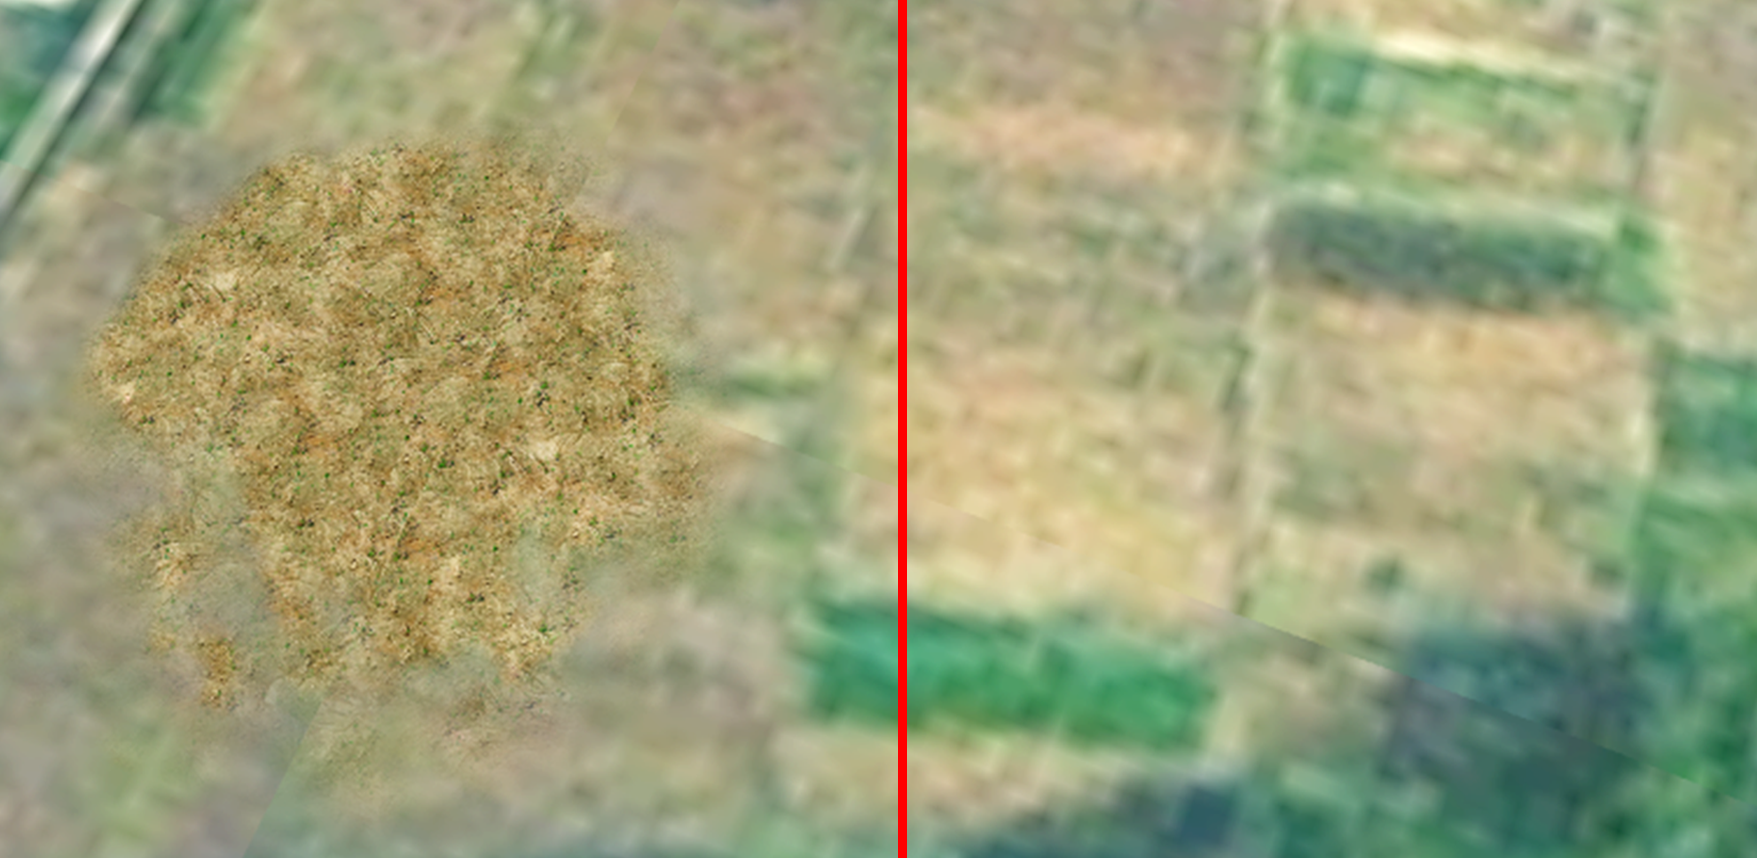
\includegraphics[height=3.3cm,width=6.3cm]{figures/groundComp.png}}
    \subcaptionbox{}{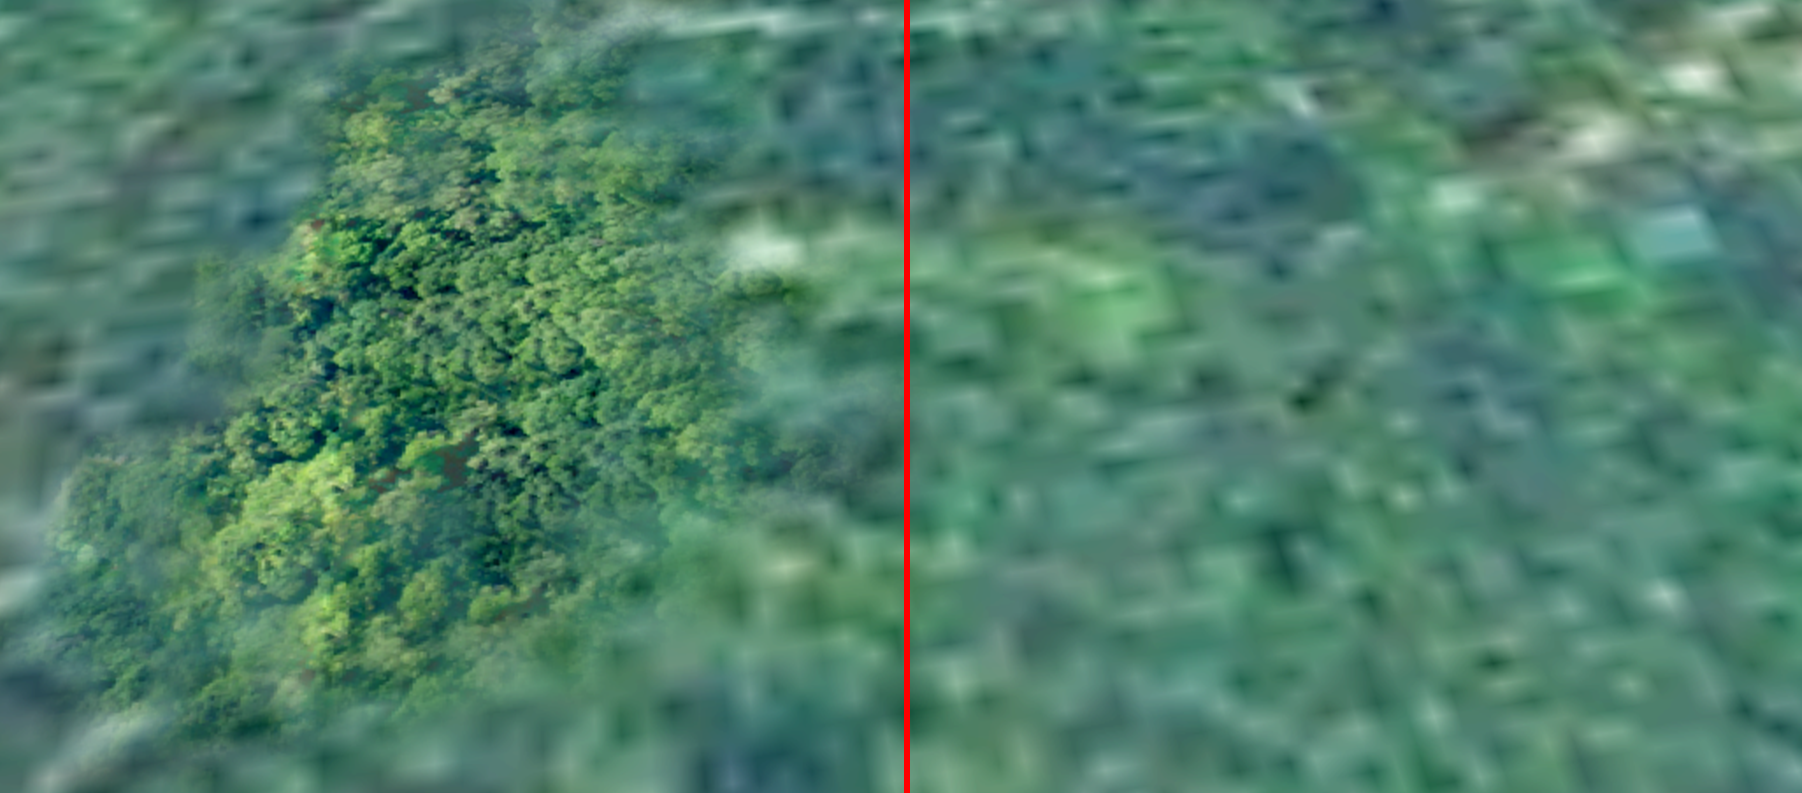
\includegraphics[height=3.3cm,width=6.3cm]{figures/treecomp2.png}}
\caption{纹理编辑结果与卫星影像精细度对比:(a).田地效果对比(b).林地效果对比}
\end{figure}
本编辑器中,纹理材质来自人工挑选制作的无缝平铺贴图,透明度贴图则通过绘制生成,并称为蒙版。有多种纹理材质参与编辑,其纹理混合结果按顺序叠加显示,因此以图层的概念对多种纹理材质的编辑进行管理,每个图层使用一个材质。在GPU中将多种纹理材质按照蒙版提供的透明度融合后,将颜色叠加到地形纹理的颜色上。本节介绍基于笔刷生成蒙版数据的方法及蒙版数据的管理。

\subsection{栅格化笔刷应用策略}
笔刷数据由函数计算得到,其值域在$[0.0,1.0]$之间,表示该像素上笔刷的作用强度,以一维数组方式存储,但看作宽高相等的二维数组。编辑时,笔刷数据与蒙版数据中的像素是一一对应关系,如笔刷直径为$n$,则笔刷投影到蒙版数据上,覆盖$n*n$的像素,对此范围内的像素产生编辑效果。需要注意的是,由于地球经线在两极处收拢,因此纬线间距离相等而经线间距离不定。在计算笔刷数据时,为了在全球各个位置保持笔刷形状固定,需要根据笔刷的宽度和笔刷所在经纬度,对笔刷的高度进行校正。取笔刷所在地形块的四个角点,计算其全球坐标,将地形块宽高比作为笔刷的宽高比,然后进行笔刷数据计算。\par

与高程编辑笔刷不同,纹理笔刷是栅格化的,与纹理蒙版像素相对应,如图5.2所示。因此相机视角变换时,分层四叉树改变造成地形块层级变换,笔刷的覆盖面积也会随纹理蒙版数据分辨率的增加而变小,产生跳变。为保证笔刷大小的统一性,避免笔刷在换层时跳变,在系统中按固定层级绘制笔刷,该层级记为$L_r$。用固定层级绘制笔刷,保证了笔刷的绘制和其直径的调整在任意视角、任意层级上都连续,但编辑时还需使笔刷层级与当前编辑层级相一致。用两个一维数组存储用于绘制和用于编辑的笔刷数据,分别记为$B_r$和$B_e$,并分别提供获取和设置该数据的接口。当将笔刷绘制到画面中的地形表面时,根据笔刷直径和当前选中的笔刷的序号实时计算出用于绘制的笔刷数据$B_r$。而将笔刷数据用于编辑时,首先获取编辑层级,即当前分层四叉树中最精细的层级,记为$L_e$,按$L_e/L_r$的比例对笔刷直径进行缩放后再计算笔刷数据,保证编辑使用的笔刷数据与绘制使用的笔刷数据覆盖的面积大小相同。\par
\begin{figure}[htb]
    \centering
    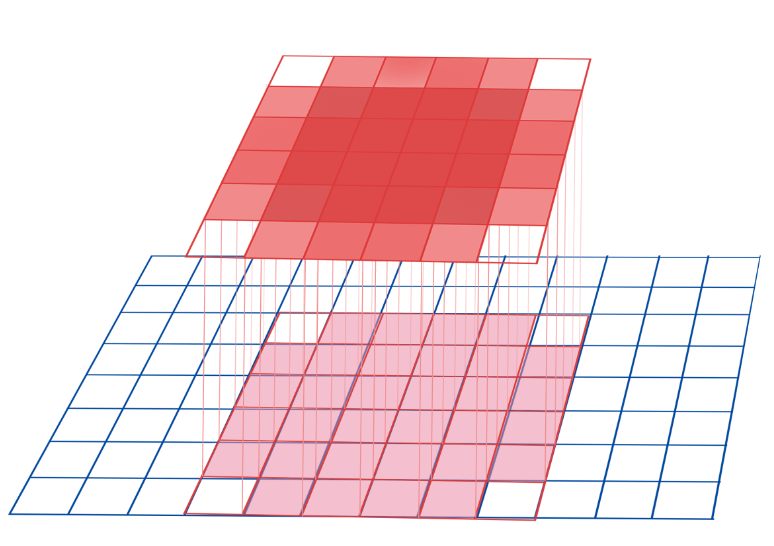
\includegraphics[height=4cm ,width=4cm]{figures/brush2.png}
  \caption{笔刷数据和蒙版数据像素一一对应}
  \end{figure}
%\begin{figure}[htb]
 %   \centering
 %   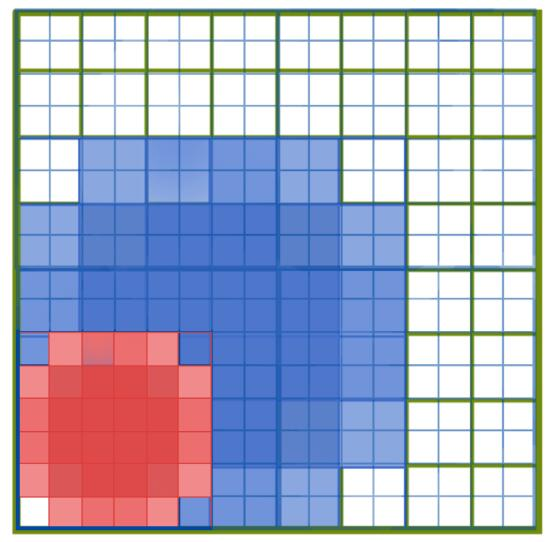
\includegraphics[height=5cm %,width=5cm]{figures/brushChange.jpg}
 % \caption{地形块换层时产生的笔刷跳变}
 % \end{figure}
  %
目前系统中分层四叉树的最高分裂层级为17层,记为$L_m$,笔刷绘制层级$L_r$为14层,考虑到计算笔刷编辑数据时对笔刷直径的调整,笔刷数据数组的宽和高(记为$n_{array}$)和可设置的最大笔刷直径(记为$n_{max}$)有如下关系:
\begin{equation}
n_{array}=(L_m/L_r)*n_{max}
\end{equation}
则存储笔刷数据的一维数组大小为$n_{array}*n_{array}$,并将其看作一个长宽均为$n_{array}$的二维数组,根据笔刷直径大小和当前选中的笔刷ID计算笔刷数据。\par
\subsection{蒙版及图层管理}
纹理编辑效果的呈现涉及图层信息和指导纹理材质混合的蒙版信息。图层信息与用户界面、配置文件等多个其他部分关系密切,因此设计为全局变量。蒙版信息与地形高程数据和纹理数据等价,是与地形块一一对应的,并以相同的方式管理和调度,挂载在四叉树的地形块节点内。\par
每个蒙版数据块内分别为每个图层提供一个数据分辨率与地表纹理数据相同的数组,该数组以智能指针进行管理,数组内每个图层的数据也以智能指针的形式管理,请求到某个图层时才为其分配内存。蒙版数据可能由父节点赋给其子节点临时使用,使用智能指针避免了内存无法正确释放的问题。蒙版数据内的像素都与地表纹理数据中的像素一一对应,每个图层在每个像素的位置用一个字节存储一个取值范围为$[0,255]$的整数值,表示该像素上对应图层的纹理材质参与颜色混合的强度,绘制时以纹理数组的形式发送给GPU。\par
图层信息包括图层名和图层使用的纹理材质。编辑器为载入的每种纹理材质生成唯一的纹理ID作为句柄,对于简单材质和复合材质是无差别的。用户界面也通过记录纹理材质选项的纹理ID,将用户所选择的纹理赋给图层。绘制时,图层所使用的纹理材质以纹理数组的形式发送给GPU,并在用户改动图层信息后设置脏标识,以向GPU传递新的纹理材质。目前系统最多允许八个图层,即可以同时使用八种纹理材质进行绘制。\par
编辑过程中有时由于调整了编辑意图,会需要抛弃整个图层的编辑结果,对图层进行删除是一种很自然的操作。删除图层涉及对多个部分数据的修改:在图层管理器中,需要将后面的图层依次前移覆盖待删除图层信息,并更新用户界面;在过滤器中,需要删除基于该图层的补丁数据;对LRU缓存中的全部蒙版缓存块,需要保留指向待删除图层蒙版数据的智能指针,将后面图层在数组中的位置前移,将待删除图层的指针放在前移后出现的空缺处。
%由于删除图层后需要向GPU传递这种更新,因此不能释放被删除图层的内存,而需要将其重置为0。
\subsection{复合纹理材质}
目前系统中的海面由高程值为0的均匀四边形面片绘制,通过噪声计算对网格点进行偏移形成海洋波浪效果。而内陆的水体如河流、湖泊等,是通过编辑工具改变地形高程值,使地形高度低于海平面,暴露出海洋网格而产生的。这种实现方式存在几个问题:(1)编辑工具产生一条折线作为河道中心线,对地形高程进行修改,产生的河道是等宽的,效果较为僵硬、不自然,尤其在河道中心线发生大角度转折时容易产生断裂;(2)距离较远观看时由于数据分辨率问题,河岸产生非常大的锯齿效果;(3)这种方法无法表现存在高度变化的水体,如从沿着山体坡度流下的河流,或高原湖泊等。图5.3示意了上述的三个问题。
\begin{figure}[htb]
    \centering
    \subcaptionbox{}{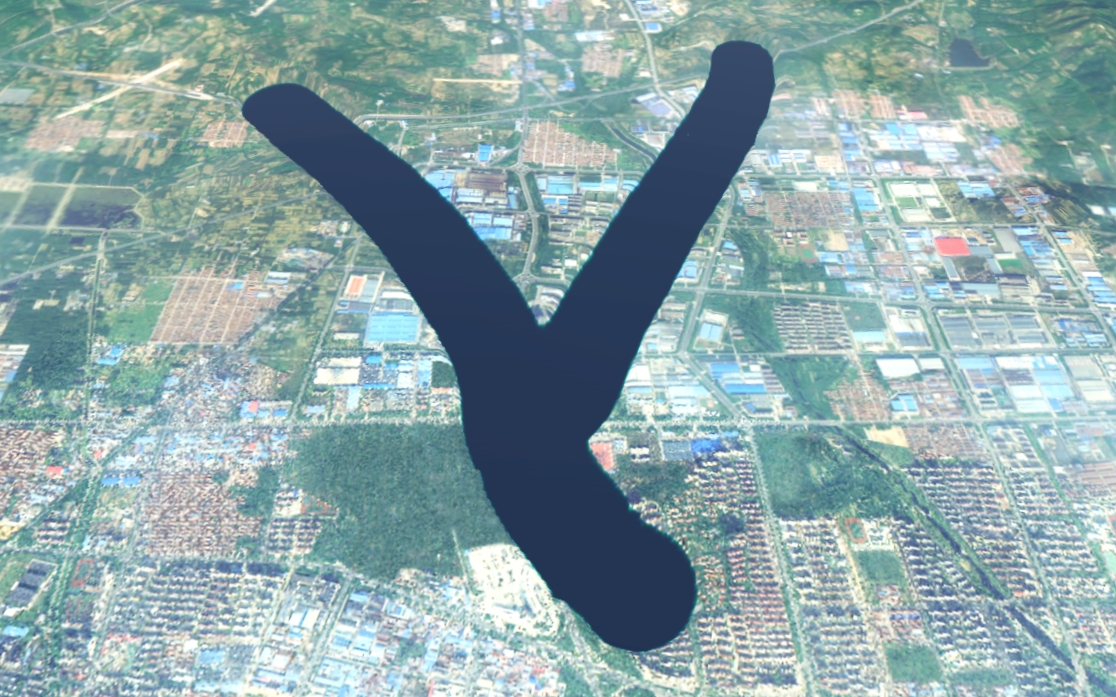
\includegraphics[height=3.7cm,width=5.3cm]{figures/riverLow.PNG}}
    \subcaptionbox{}{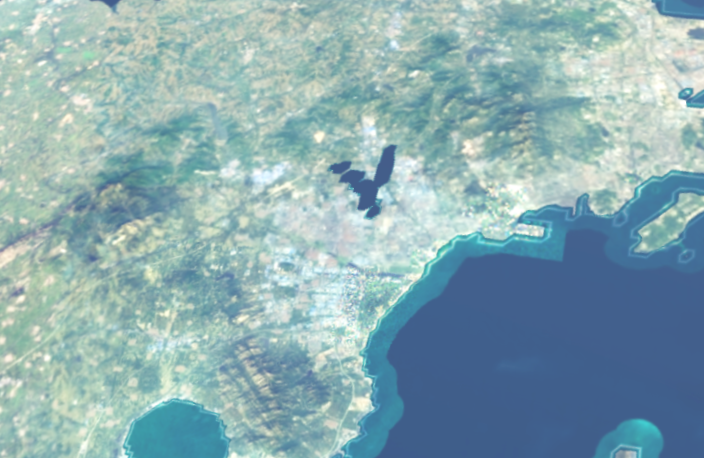
\includegraphics[height=3.7cm,width=5.3cm]{figures/riverHigh.PNG}}
    \caption{通过地形高程编辑实现的河流在高空视角出现严重的锯齿:(a).低空视角(b).高空视角}
\end{figure}
因此,用纹理编辑的方式对水体编辑进行改进成为了自然的想法。水体一个重要的视觉特性就是其对太阳光的高光反射。为使水体产生高光反射,需要向着色器中传入水面材质的法线信息,由此引出了构造复合材质的需求。\par
将只有颜色贴图的单一资源的纹理材质扩充为包含颜色贴图、法线贴图等资源的复合纹理材质,可以创建更复杂的地表纹理编辑效果。但只有颜色贴图的简单材质依然非常方便实用,复合材质和简单材质需要同时应用在系统中。在本地的配置文件中对复合材质所需的多种贴图资源路径进行配置,并在着色器中增加一个变量用于表示当前材质所包含的资源种类,以在着色器中同时对包含不同资源的纹理材质进行统一处理。以复合材质实现的内陆水体效果如图5.4所示:
\begin{figure}[htb]
    \centering
    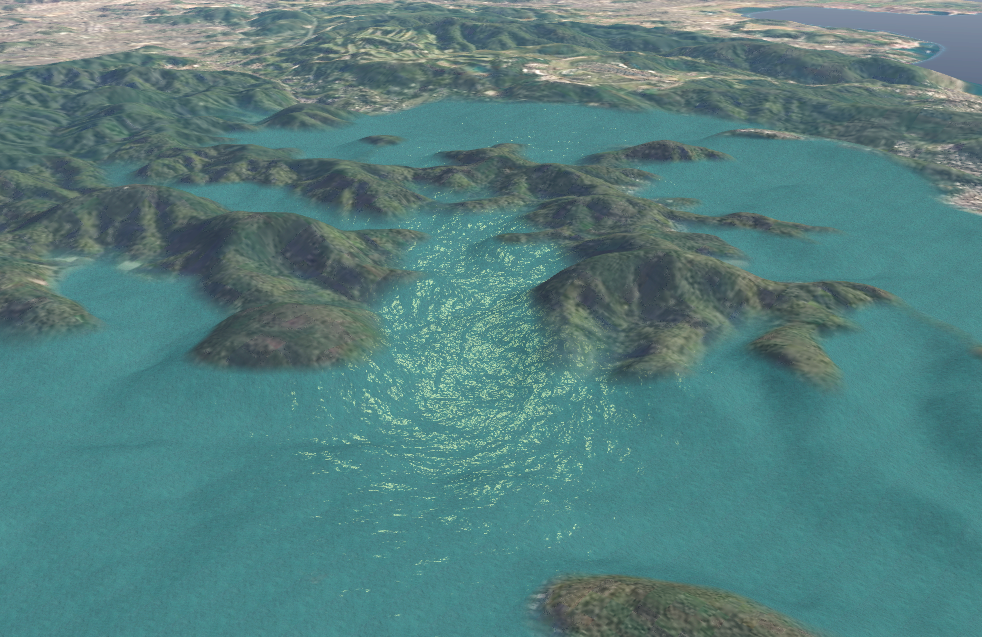
\includegraphics[height=6cm,width=9.4cm]{figures/water.png}
    \caption{复合材质和基于高程规则的纹理笔刷实现的内陆水体}
\end{figure}
\subsection{基于高程规则的过程式纹理笔刷}
积雪和植被等地物存在垂直分布规律,高程数据所表达出的地貌通常应与地面纹理表达的内容相对应。尽管受到地理位置和气候等因素影响,且不同地形的垂直分布存在差异,但总的来说积雪、植被等地物分布呈现一定规律。基于对自然界地景规律的观察,用地形的海拔高度、斜率等数据作为笔刷编辑的辅助约束成为了很自然的想法。\par
将对笔刷编辑结果的约束条件称为过程式编辑规则,需要在配置文件设置的参数包括过程式编辑规则的名称、地形高度、地形斜率、过渡带宽度等。进行笔刷编辑时,如未选中过程式编辑规则或处在橡皮擦模式,则不做处理。当选中过程式编辑规则时,编辑曲线绘制工具在创建纹理蒙版补丁数据的同时,还需要创建一块等大的高程补丁数据,并拷贝原始高程数据进行填充。同时由于该过程式编辑规则只应用在单条笔迹上,不能对整个地形块蒙版数据的其他部分产生影响,需要将本次编辑的笔迹与之前的编辑痕迹区分开,因此还需要创建一块等大的空白的补丁数据,用于接受本次的编辑结果。\par
首先,按照原有的编辑流程通过笔刷绘制点和笔刷模板生成编辑结果。对于不应用过程式编辑规则的编辑笔迹,直接修改到蒙版补丁数据上,对于应用过程式编辑规则的编辑笔迹,则先修改到空白补丁数据上。与高程编辑不同,纹理编辑的笔刷编辑结果计算无需采样现有的数据,笔迹之间编辑效果是独立的,因此可以保证先将编辑结果应用到空白补丁数据上,再合并回蒙版补丁数据的正确性。当一条笔迹绘制结束时,在将编辑结果向各地形块数据分发之前,首先对编辑出的补丁数据应用过程式编辑规则。将编辑生成的补丁数据和高程补丁数据传输到GPU端,类似地形选区编辑,将补丁数据渲染到一个四边形面片上,在片元着色器中应用过程式编辑规则。对于补丁数据中的每一个像素,其初始透明度为1.0,按顺序应用过程式编辑规则中的多个约束条件,如高程约束、斜率约束等,每个约束条件依次对透明度值进行修改。过渡带在高程约束计算中的应用如图5.5所示,红色的两条线表示用户自定义配置的高度上限和下限,橙色线表示过渡带上边界和下边界,红色和橙色线间的部分表示过渡带,其宽度也由用户定义,过渡带可以使编辑结果不会出现硬边界。
\begin{figure}[H]
    \centering
    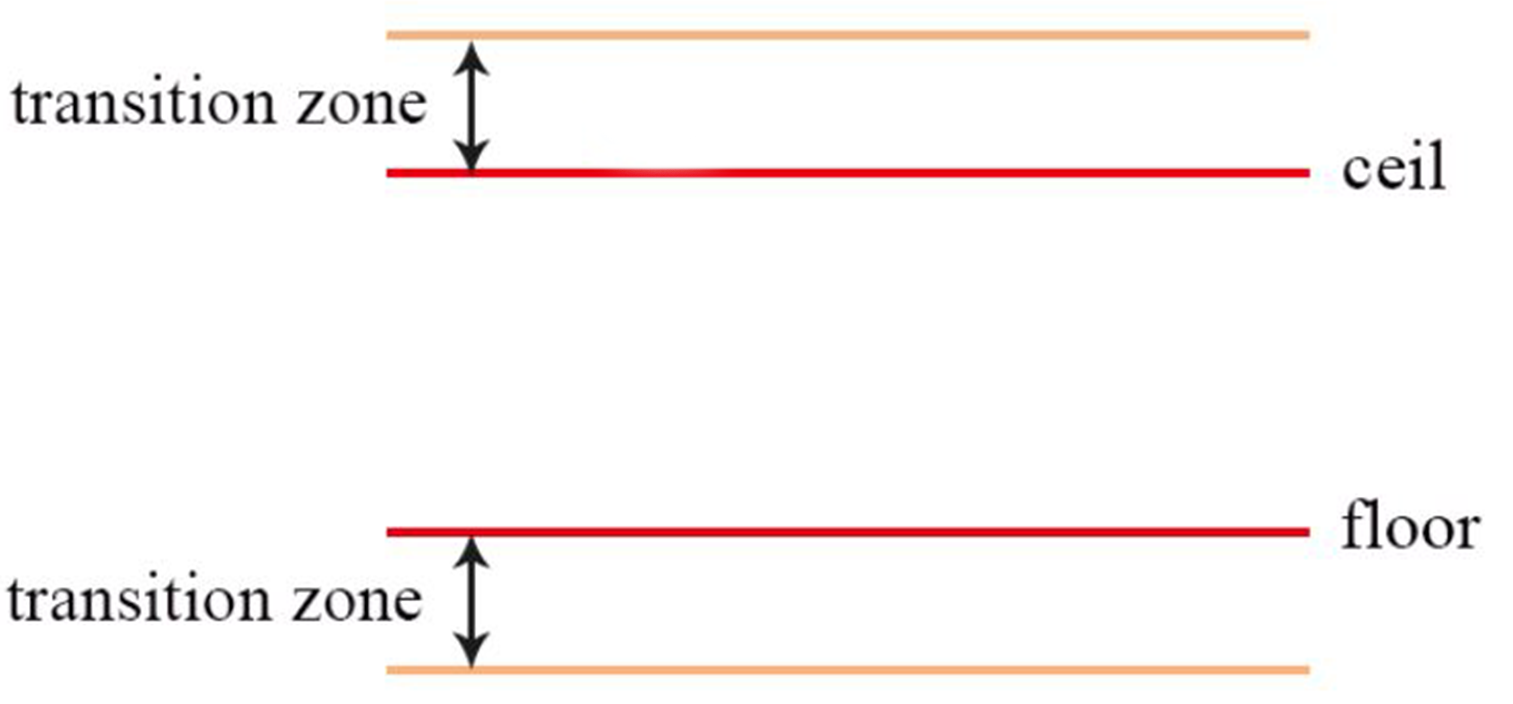
\includegraphics[height=3.4cm ,width=6.3cm]{figures/trans.png}
    \caption{高程规则的计算}
 \end{figure}
应用过程式高程规则的算法如下所示:\par
 \begin{algorithm}[H]
	\renewcommand{\algorithmicrequire}{\textbf{Input:}}
	\renewcommand{\algorithmicensure}{\textbf{Output:}}
	\caption{过程式高程规则应用算法}
	\label{alg:1}
	\begin{algorithmic}[1]
		\REQUIRE 地形高程$H$,地形斜率$G$,高程规则$R_h$,斜率规则$R_g$,过渡带宽度$T$,过渡带硬度$S$,算法强度$I$
		\ENSURE 蒙版补丁数据透明度$opacity$
		\STATE 设置$opacity$为1.0
	    \IF {$H$ > $(R_h.ceil+R_h.floor)/2$}
	    \STATE 设置$opacity$为$opacity$与$(R_h.ceil+T-M_d)/(T*S)$的乘积,并截取在[0.0,1.0]之间
	    \ELSE 
	    \STATE 设置$opacity$为$opacity$与$(M_d-R_h.floor+T)/(T*S)$的乘积,并截取在[0.0,1.0]之间
		\ENDIF
		\IF {$G$ > $R_g.floor$且$G$ < $R_g.ceil$}
	    \STATE 设置$opacity$为$opacity$与1.0的乘积
	    \ELSE 
	    \STATE 设置$opacity$为$opacity$与$(1-I)$的乘积
		\ENDIF
		\STATE \textbf{return} $opacity$
	\end{algorithmic}  
\end{algorithm}
图5.6和5.7展示了上述算法的应用效果:
\begin{figure}[H]
    \centering
   \subcaptionbox{}{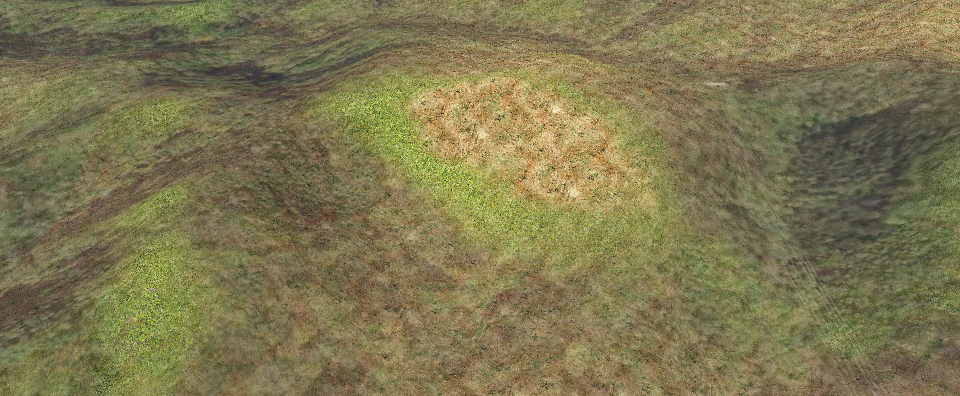
\includegraphics[height=4cm,width=5.5cm]{figures/gradient2.PNG}}
   \subcaptionbox{}{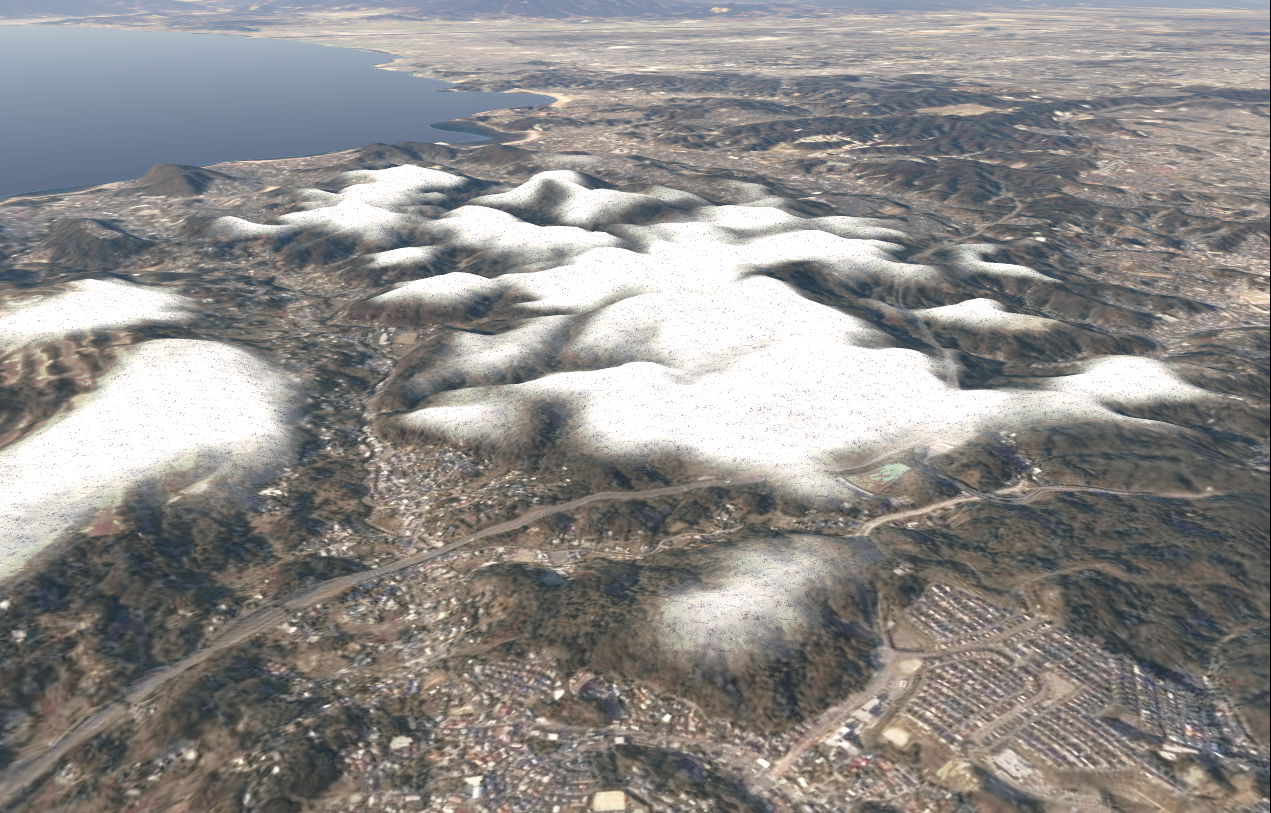
\includegraphics[height=4cm,width=5.5cm]{figures/pc-snow.png}}
  \caption{使用过程式编辑规则的纹理笔刷效果:(a).通过斜率约束绘制山坡陡峭处的地表裸露(b).通过高程约束和斜率约束实现山顶积雪效果}
\end{figure}
  
\begin{figure}[H]
    \centering
    \subcaptionbox{}{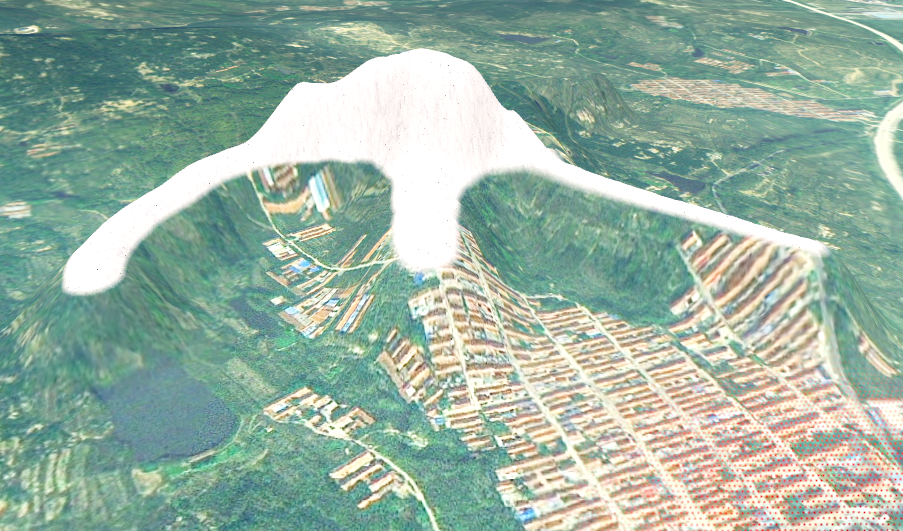
\includegraphics[height=3.2cm,width=5.2cm]{figures/110-0-35.PNG}}
    \subcaptionbox{}{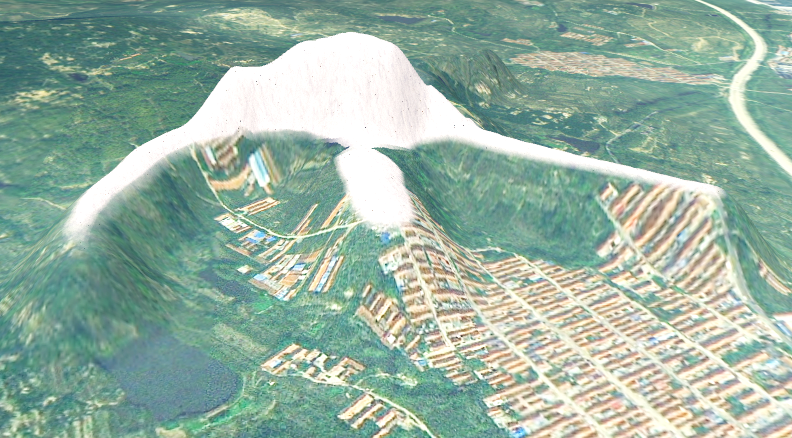
\includegraphics[height=3.2cm,width=5.2cm]{figures/110-0-19.PNG}}
    \subcaptionbox{}{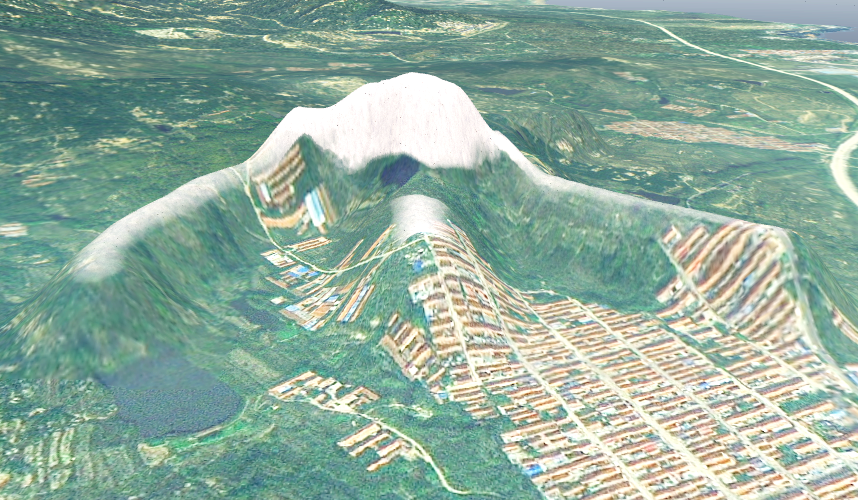
\includegraphics[height=3.2cm,width=5.2cm]{figures/110-0-13.PNG}}
    \caption{高程规则参数调整效果:高程下限:110.0,斜率下限:0.0(a).斜率上限:13.0(b).斜率上限:19.0(c).斜率上限:35.0}
\end{figure}

\section{纹理细节增强}
目前ViWo系统使用的卫星数据是由日本METI和美国NASA联合研制的ASTER-GDEM-V2数据集,其水平精度为30米,垂直精度为20米。受数据精度限制,漫游视角靠近地表时纹理看起来非常模糊,若直接将建筑模型置于缺乏细节的地表上,近距离观看时真实感较差。本文参考Genesis\supercite{genesis}等飞行视景模拟器的近地表效果,实现了基于粗糙影像的纹理合成,对低分辨率的地表纹理的颜色信息进行分析,以贴花技术为地表纹理增添细节。本方法的有效性和可行性基于对以下三点的考虑:(1)颜色是在图像处理中应用最广泛的视觉特征值,颜色包含的信息往往与图像中物体或场景的语义信息十分相关;(2)相比其他视觉特征,颜色信息对图像本身的尺寸、方向、视角的依赖性较小,提取颜色信息进行语义分析具有较高的鲁棒性;(3)本方法在片元着色器中对片元颜色进行简单处理,时间及空间开销非常低。\par
对颜色信息进行分析时,在不同的色彩空间进行处理分析的效果不同。颜色可以用一维、二维、三维和四维空间坐标表示,定义颜色的色彩空间有很多种,常用的有RGB、CMYK、HSV等。RGB色彩空间的特点之一是其三个通道的数值都容易随图片亮度改变,使结果颜色的明暗发生变化,但色调并不会产生很大变化。而往往一个通道的轻微改变,会导致最后融合在一起的颜色发生很大变化。HSV色彩空间可以较好地把颜色信息和亮度信息分开,将它们放在不同的通道中,减小了光线强度对于特定颜色识别的影响,在图像处理领域很常用。但经过实际测试,由于可能为植被的区域跨越的色环角度较大,在HSV色彩空间进行阈值分割的效果不够好,因此本文选择在RGB色彩空间进行颜色分析。由于RGB色彩空间受颜色亮度影响强烈的特性,因此不能简单的基于RGB色彩空间中某个通道的固定阈值对颜色进行判断,但可以以红、绿、蓝三种光的相对占比作为衡量的标准之一。\par
虚拟地球漫游中用户比起海洋更加关注陆地区域,陆地区域中最关注的地形语义以城市和城市周边自然环境为主,其中自然环境以植被覆盖的地形和土地、荒地为主,城市地物以建筑屋顶、道路为主。本文实现中以森林绿、泥土棕、建筑灰三种颜色对上述三种区域进行语义分割,并在渲染时在相应区域添加对应的细节,基本可以满足对地表纹理的细化需求。算法的主要思想是检查片元颜色是否较强烈的指向某种语义。如果是,则完全的使用对应语义的贴花纹理,否则对多种贴花纹理进行混合。森林绿和建筑灰在语义上强烈的指向植被和建筑屋顶,可以认为有这样颜色的像素语义较为清晰。而其他颜色的像素可能是由于图像分辨率低和卫星影像阴影问题,导致语义较为模糊。选择具有普适性的泥土的细节纹理作为两个区域间的过渡,在不明确是植被也不明确是建筑的部分进行细节纹理的混合。需要注意的是,纹理编辑后对地表纹理的语义信息也施加了改变,在着色器中可以得到从卫星影像采样和纹理编辑结果叠加后的像素颜色,将该颜色用于判定。算法输入片元颜色,输出三种细节纹理的alpha值,作为进行细节纹理混合的依据,最后将细节纹理叠加到原有的片元颜色上。为使细节只在近地漫游时出现,该算法在高空视角和低空视角呈现差异,根据当前四叉树中的最精细层级对细节纹理的透明度进行调整。
算法详细流程如算法2所示,图5.8从高空视角展示了语义划分的结果,并从近地面视角展示了贴花应用结果。

\begin{algorithm}[h]
	\renewcommand{\algorithmicrequire}{\textbf{Input:}}
	\renewcommand{\algorithmicensure}{\textbf{Output:}}
	\caption{基于粗糙卫星影像的贴花纹理alpha值计算}
	\label{alg:1}
	\begin{algorithmic}[1]
		\REQUIRE 卫星影像采样颜色$C_s$,当前四叉树最精细层级$l$
		\ENSURE 植被细节纹理alpha值$A_g$,建筑细节纹理alpha值$A_b$,泥土细节纹理alpha值$A_s$,细节纹理总体alpha值$A_m$
		\STATE 设定细节纹理最小混合层级$l_{min}$和最大混合层级$l_{max}$,砖石颜色$C_b$,植被细节纹理阈值$t$,建筑细节纹理阈值$s$
		\STATE 将$A_m$设置为$l$-$l_{min}$的倍数,并截取其值在$[0.0,1.0]$
		\STATE 将$sum$设置为$C_s$三个通道值的和
		\STATE 将三元量$contrib$设为$C_s$三个分量与$sum$的比值
		\STATE 设置$A_g$为$contrib.g$的两倍并截取其值在$[0.0,1.0]$
		\STATE 设置$A_b$为$C_s$与$C_b$的点乘
	    \IF {$A_g$ > $t$}
	    \STATE 设置$A_g$为1,$A_b$、$A_s$为0
	    \ELSIF{$A_b$ > $s$}
	    \STATE 设置$A_b$为1,$A_g$、$A_s$为0
	    \ELSE 
	    \STATE 设置$A_s$为1减去$A_g$和$A_b$结果的倍数
		\ENDIF
		\STATE \textbf{return} $A_g$, $A_b$, $A_s$
	\end{algorithmic}  
\end{algorithm}
\begin{figure}[H]
    \centering
    \subcaptionbox{}{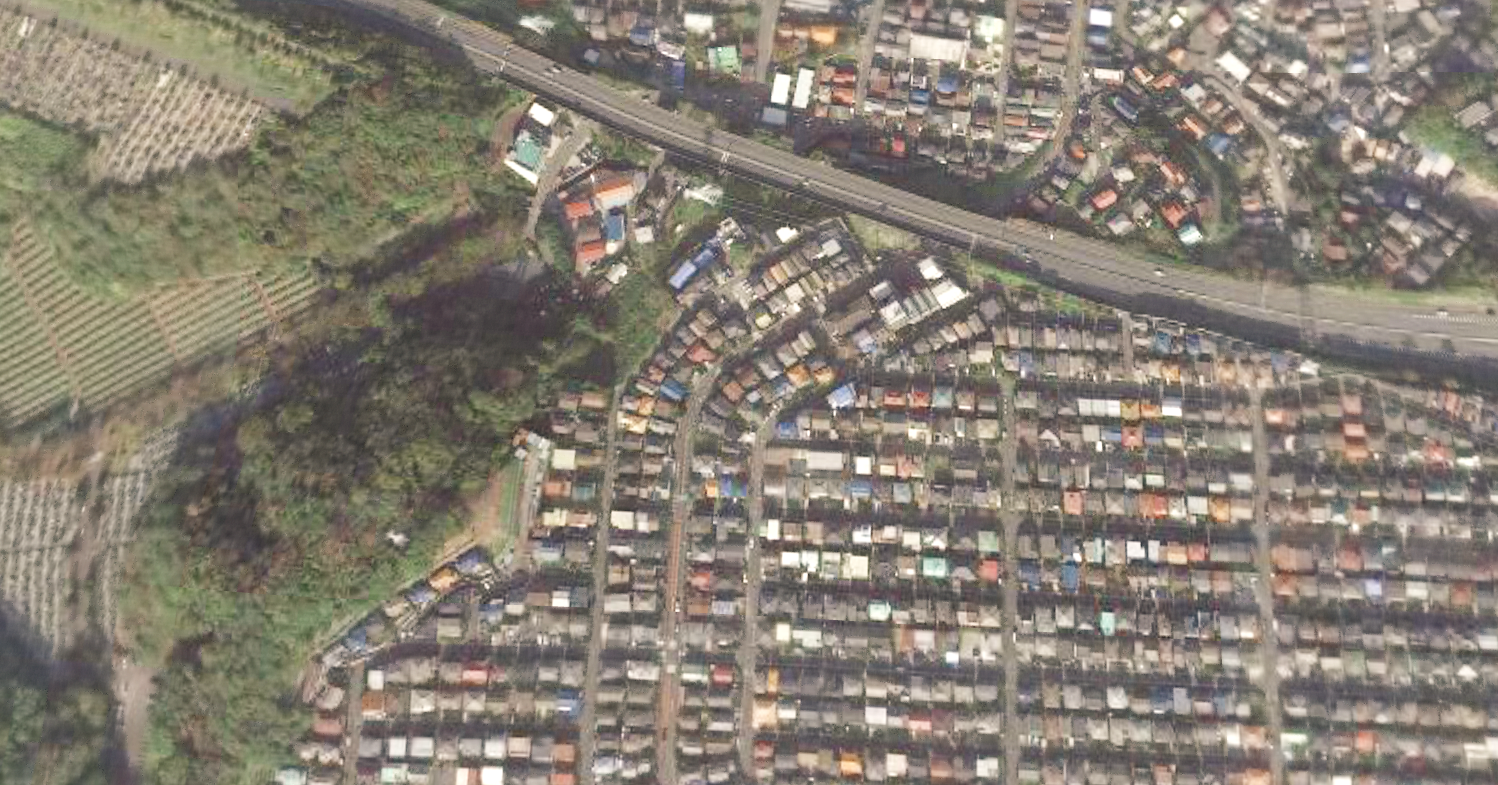
\includegraphics[height=4.3cm,width=6.4cm]{figures/origin-devide.png}}
    \subcaptionbox{}{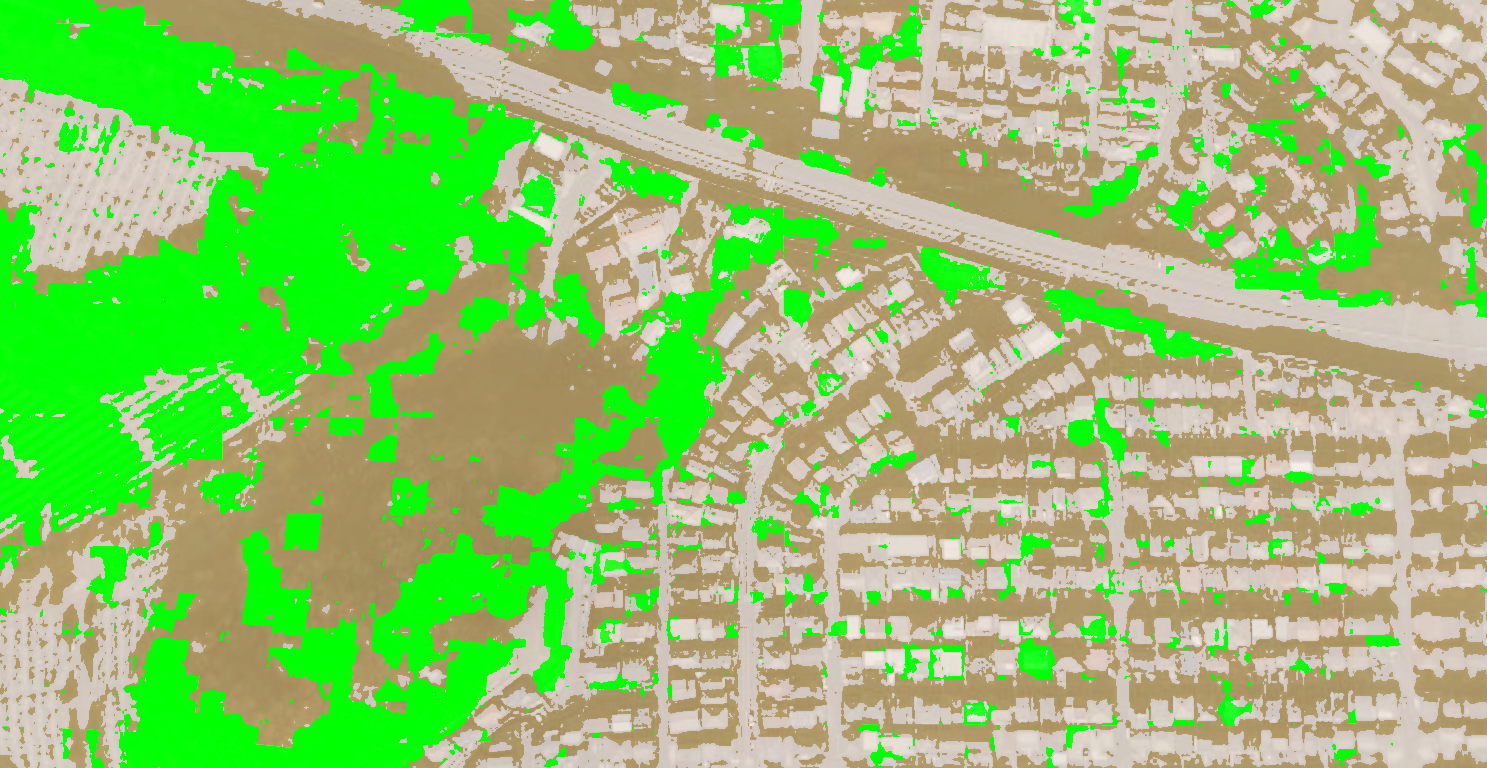
\includegraphics[height=4.3cm,width=6.4cm]{figures/devide.png}}
    \subcaptionbox{}{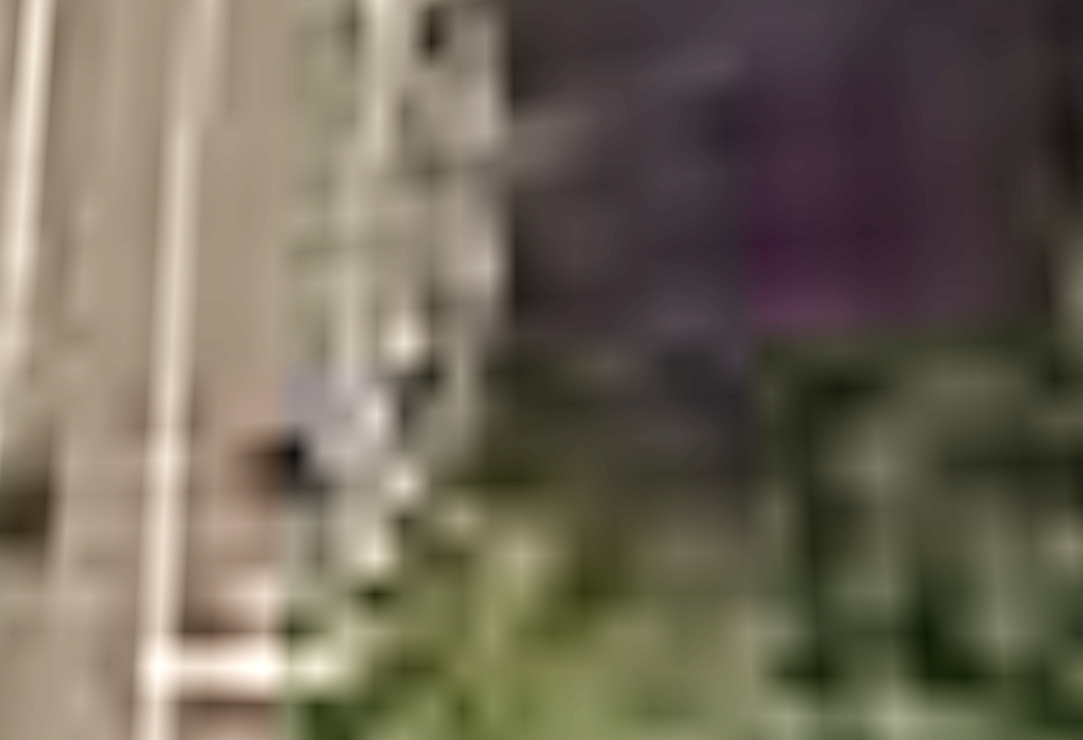
\includegraphics[height=4.6cm,width=6.4cm]{figures/beforedecal.PNG}}
    \subcaptionbox{}{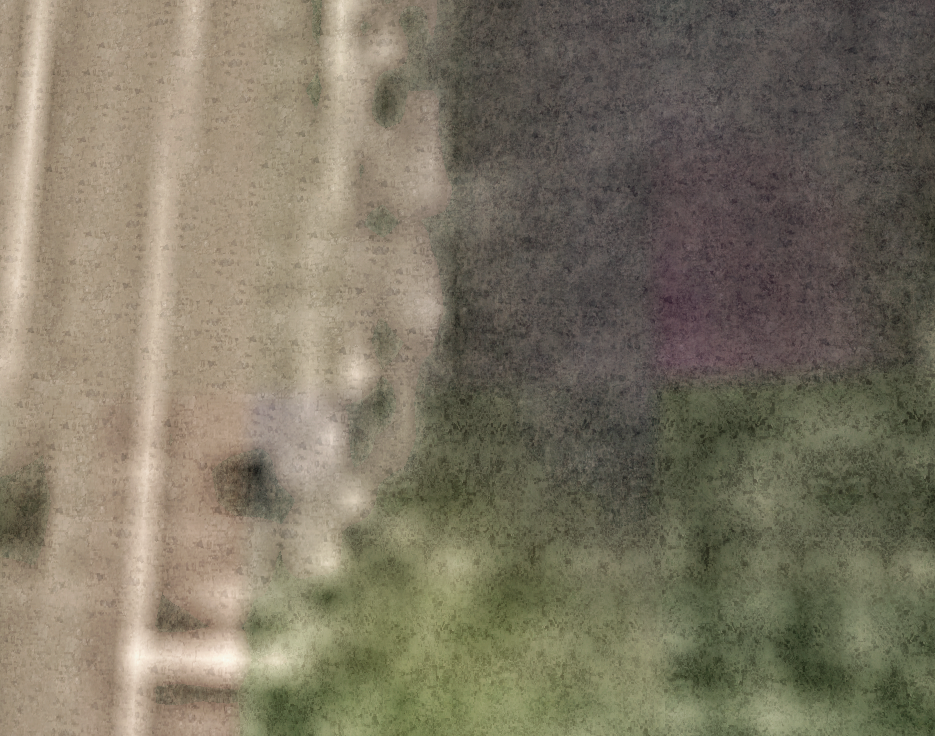
\includegraphics[height=4.6cm,width=6.4cm]{figures/afterdecal.png}}
    \caption{贴花技术应用结果:(a).原卫星影像(b).区域划分结果:绿色部分为植被,棕色部分为土地,灰色部分为建筑(c).应用贴花技术前,近地漫游时局部地表纹理非常模糊(d).贴花技术应用效果,图中可见植被、泥土和砖石不同的细节纹理}
\end{figure}
\section{卫星影像内容增强}
用卫星影像作为地表纹理构建虚拟地球存在一个局限,即卫星影像数据只能呈现特定季节的环境。对于飞行视景模拟等应用,用户希望能对多种环境进行模拟,对虚拟环境季节特征的体现是很自然的需求。从卫星影像的层面来看,季节变化过程中在图像中呈现最大变化的是植被覆盖的地区。因此对植被覆盖区域进行后处理可以很大程度的模拟不同季节的卫星影像。\par
ASTER-GDEM-V2数据集摄制于夏季,因此图片中颜色偏绿且明度低的部分很可能是植被覆盖的区域。春夏季的卫星影像特征是植被覆盖区域呈现深绿色,秋季则由于植被枯黄,在植被覆盖区域渐渐呈现土黄色、黄棕色。冬季的卫星影像特征是植被凋零,原有的绿色植被区域留下枝干和泥土,呈现深棕色。除此之外,冬季会出现积雪,覆盖除道路之外的大部分区域,真实的雪天卫星影像主要色调为白色和深棕色。图5.9展示了真实世界各个季节卫星影像的色调。
\begin{figure}[!h]
    \centering
   
     \subcaptionbox{}{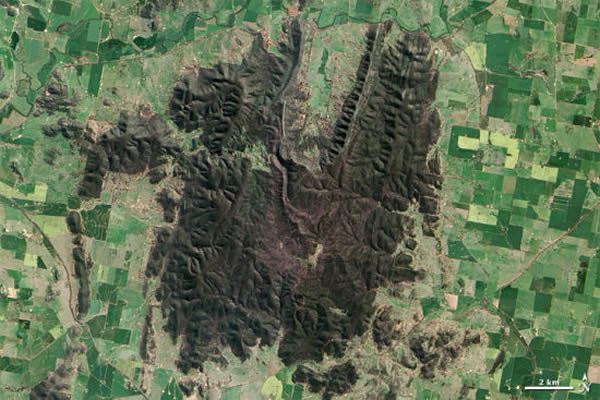
\includegraphics[height=3.5cm,width=5.25cm]{figures/1_201207311659031a5mz.jpg}}
    \subcaptionbox{}{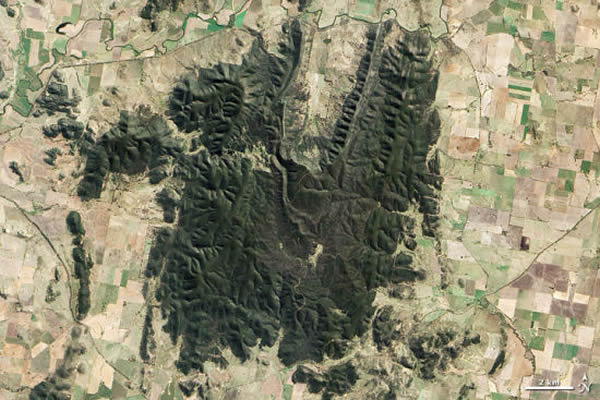
\includegraphics[height=3.5cm,width=5.2cm]{figures/1_201207311658321sgow.jpg}}
     \subcaptionbox{}{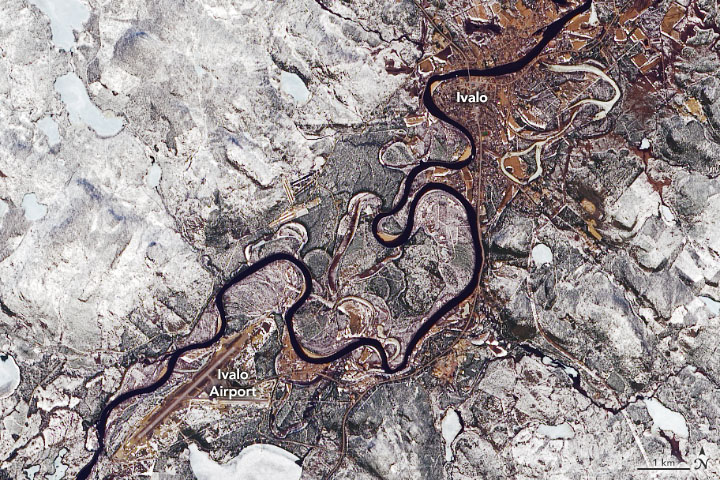
\includegraphics[height=3.5cm,width=5.1cm]{figures/ivalo_oli_2020146.jpg}}
    \caption{原始卫星影像:(a).澳洲Nangar国家公园春夏季卫星影像\supercite{nangar}(b).澳洲Nangar国家公园秋季卫星影像\supercite{nangar}(c).芬兰Ivalo机场雪天卫星影像\supercite{thaws}}
\end{figure}

算法开始前,可以手动的在真实的四季卫星影像上选取当季植被的颜色,作为目标颜色,该颜色值为本算法的输入,称为输入色。不同地区由于植被分布不同,四季中呈现的颜色变化规律也不同,根据输入色的不同,可以进行调整以达到理想的效果。本文在系统实现中为四季分别定义了调色参数,将日期折算为一个[0.0,1.0]间的浮点值,用于在四季的调色参数间平滑插值,实现了四季效果的平滑变化。考虑到低纬度地区在卫星影像中的植被颜色几乎不随季节变化而变化,因此纬度信息需要参与输入色混合权重的计算,详细算法如下:\par

\begin{algorithm}[H]
	\renewcommand{\algorithmicrequire}{\textbf{Input:}}
	\renewcommand{\algorithmicensure}{\textbf{Output:}}
	\caption{基于粗糙卫星影像的四季颜色调整算法}
	\label{alg:1}
	\begin{algorithmic}[1]
		\REQUIRE 卫星影像采样颜色$C_{in}$,当前四叉树最精细层级$l$,输入色$C_{tone}$,经纬度$lal$
		\newpage
		\ENSURE 调色后的颜色$C_{out}$
		\STATE 设置绿色的贡献度$contrib$为$C_{in}.g-(C_{in}.r+C_{in}.b)*0.5$
		\STATE 设置平均颜色强度$intensity$为$C_{in}$的三个通道的平均值
		
		\STATE 根据平均颜色强度对输入色进行调整,设置$C_{balance}$为$C_{tone}*intensity$的倍数
		\STATE 设置$lalrate$为$lal/50.0$并截取结果在[0.0,1.0]之间
	    \IF {$C_{in}$的模长小于0.68}
	    \STATE 判断$C_{in}$可能是植被覆盖区域,设置$C_{out}$为$C_{in}$与$C_{balance}$的混合,混合系数为$contrib$*$t$*$lalrate$,$t$为效果调整参数
		\ENDIF
		\IF{开启积雪覆盖效果}
		\STATE 设置积雪透明度$scale$为$contrib$与调节参数的积,并截取在$[0.0,1.0]$之间。
		\STATE 设置积雪颜色$C_{snow}$
		\STATE 设置$C_{out}$为$C_{out}$与$C_{snow}$的混合,混合系数为$scale$。
		\ENDIF
		\STATE \textbf{return} $C_{out}$
	\end{algorithmic}  
\end{algorithm}
\newpage

\newpage
\begin{figure}[H]
    \centering
    \subcaptionbox{}{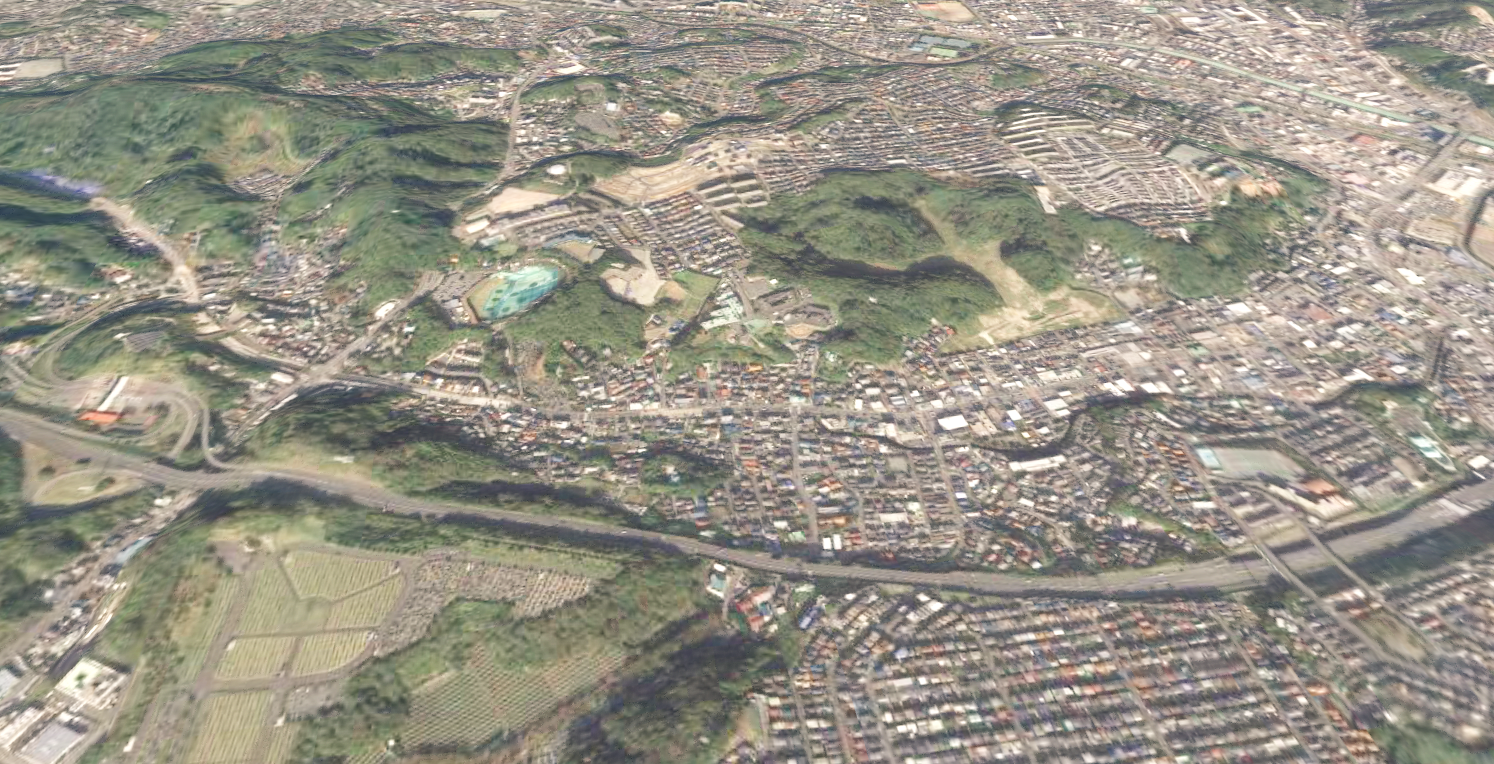
\includegraphics[height=4cm,width=5.5cm]{figures/original.png}} \\

    \subcaptionbox{}{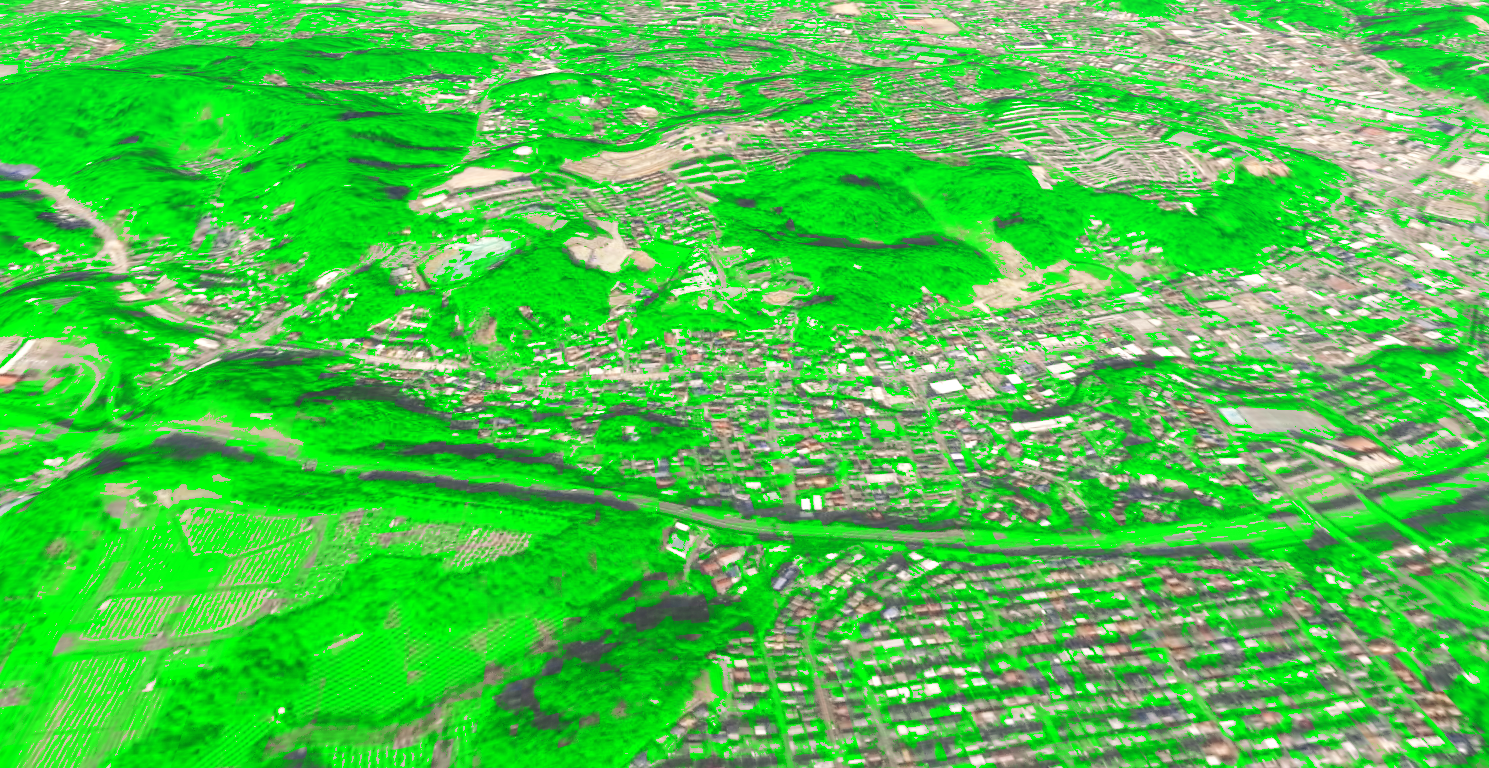
\includegraphics[height=4cm,width=5.5cm]{figures/adjustArea.png}}
    \subcaptionbox{}{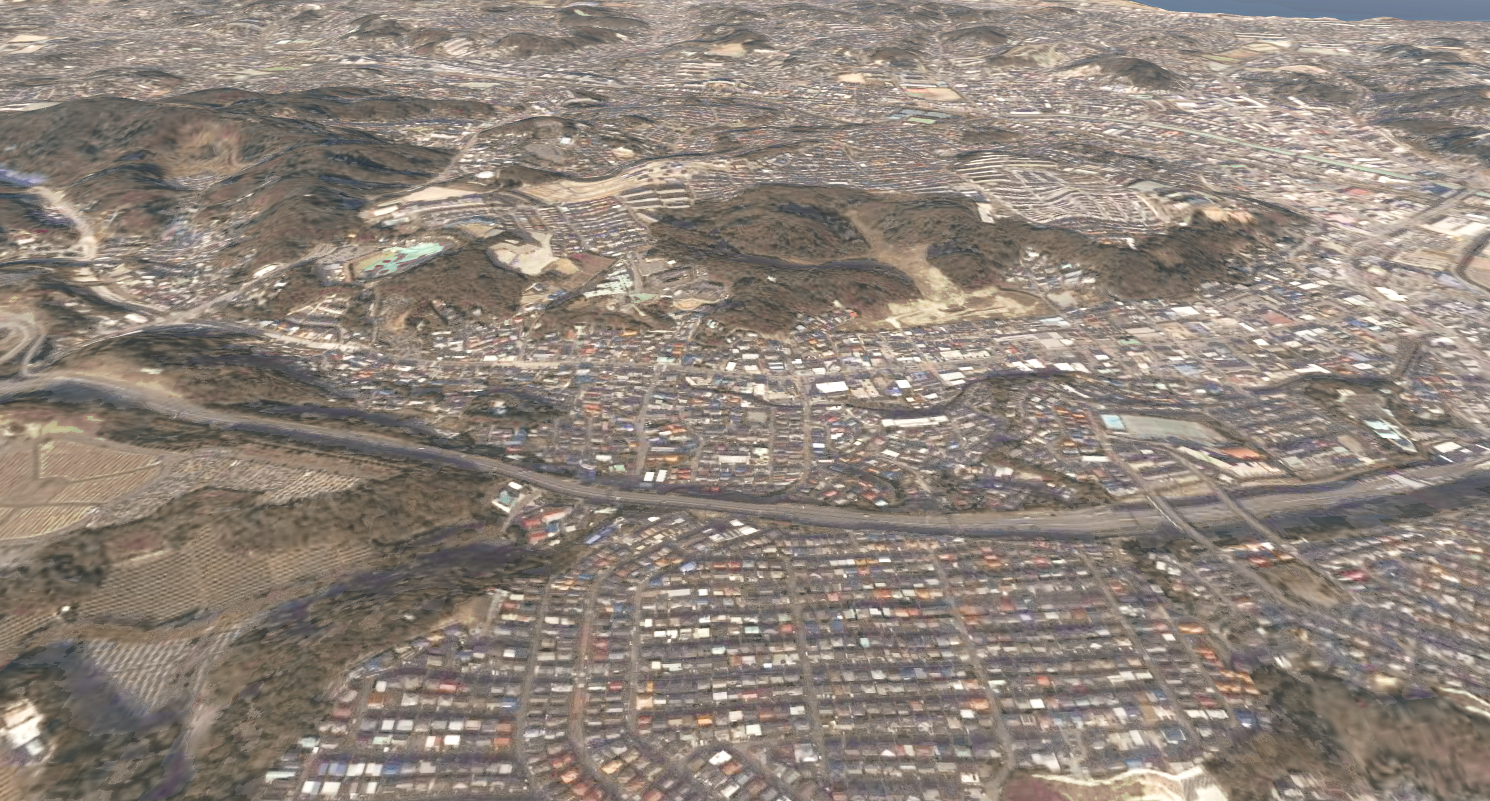
\includegraphics[height=4cm,width=5.5cm]{figures/winter.PNG}}

    \subcaptionbox{}{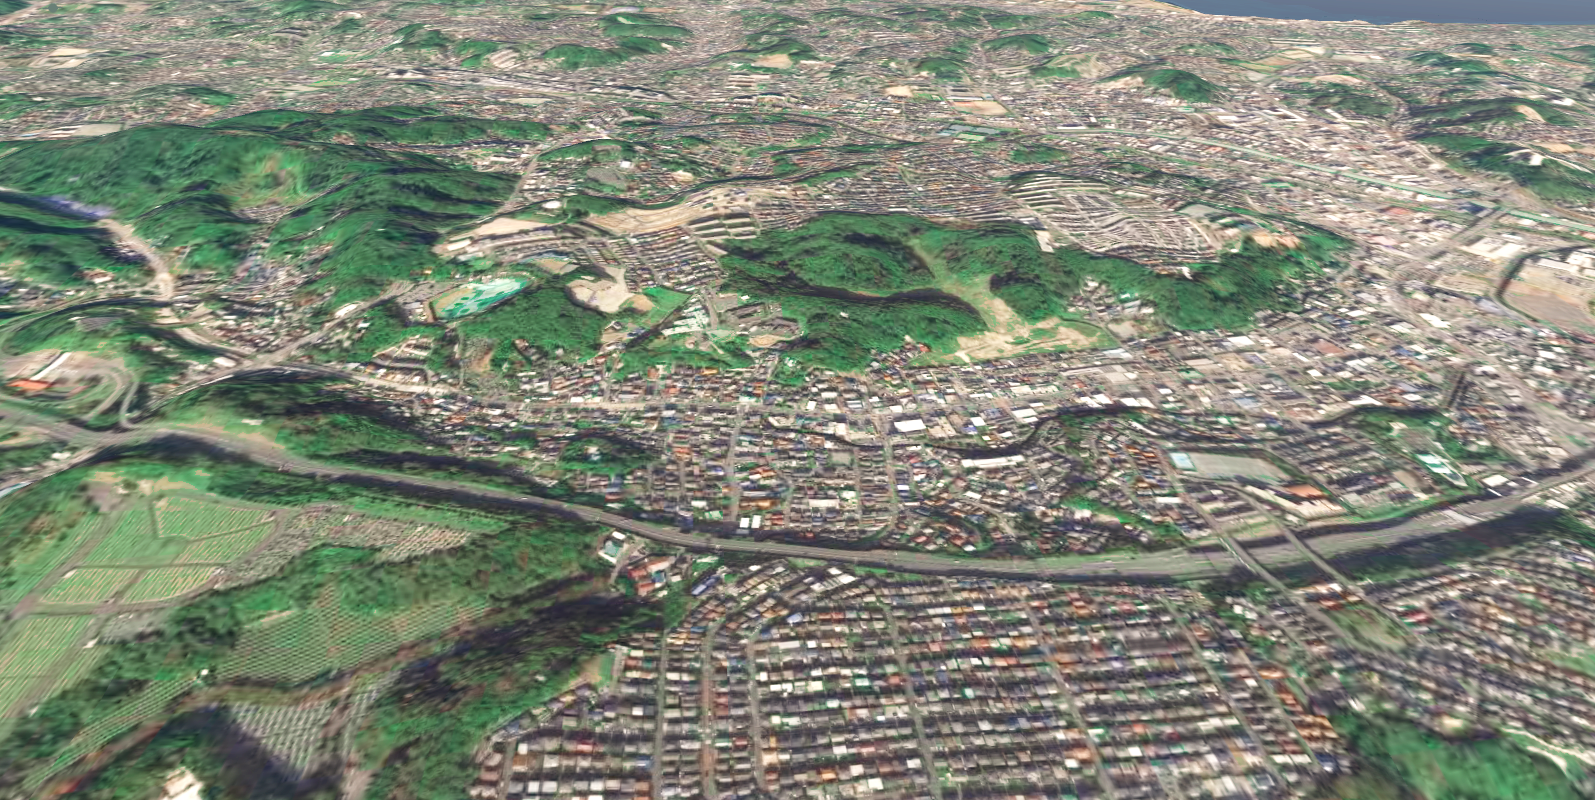
\includegraphics[height=4cm,width=5.5cm]{figures/spring2.PNG}}
    \subcaptionbox{}{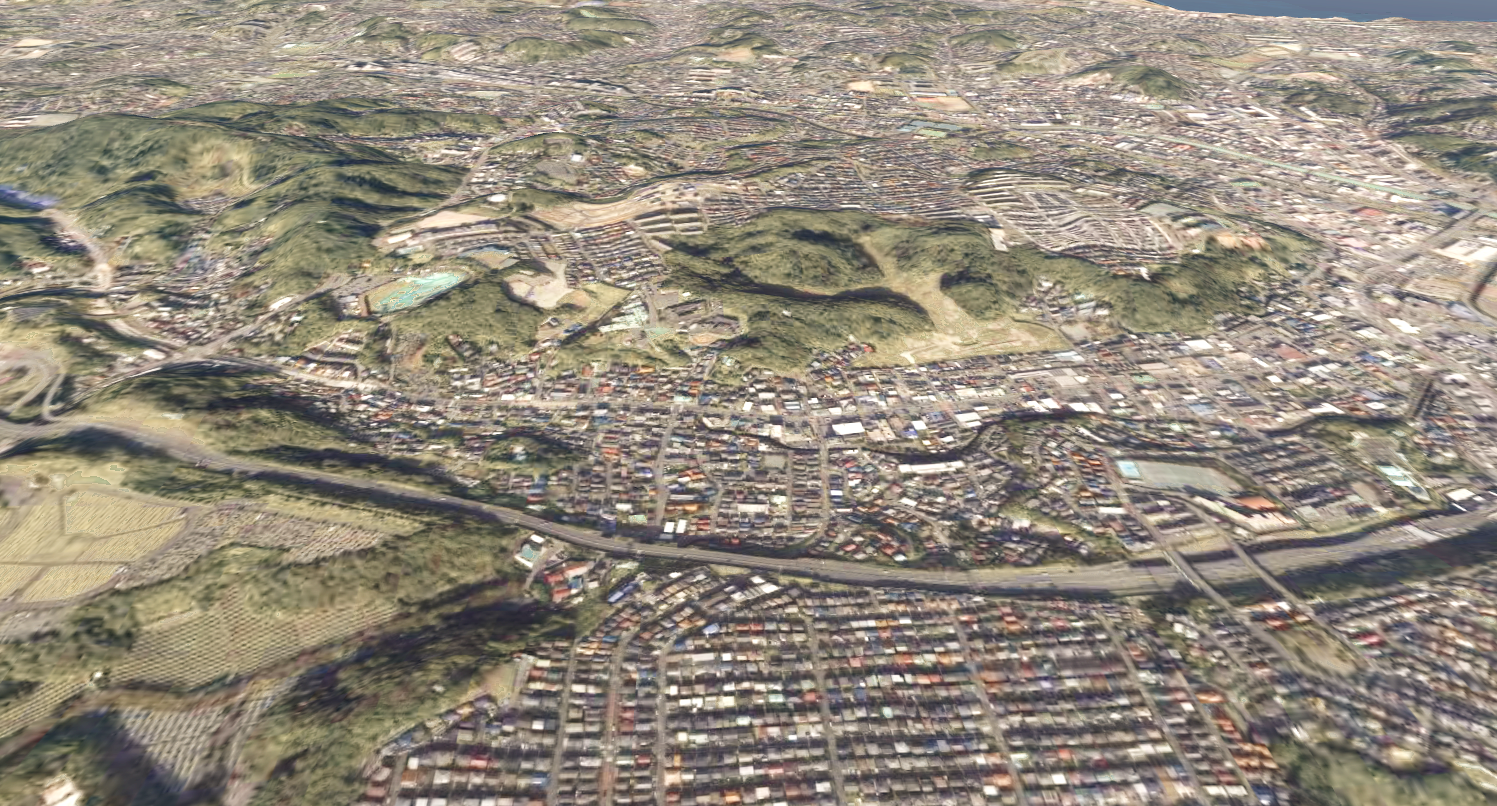
\includegraphics[height=4cm,width=5.5cm]{figures/autumn.PNG}}
    \caption{调色区域和最终调色效果:(a).原始卫星影像(b).调色区域(c).冬季调色效果(d).春夏季调色效果(e).秋季调色效果}
\end{figure}

植被覆盖的区域由于人类活动较少,更可能维持积雪覆盖的状况,因此以绿色作为衡量积雪覆盖率的一个参考值,形成的覆雪效果如图5.11所示。
\begin{figure}[H]
    \centering
    \subcaptionbox{}{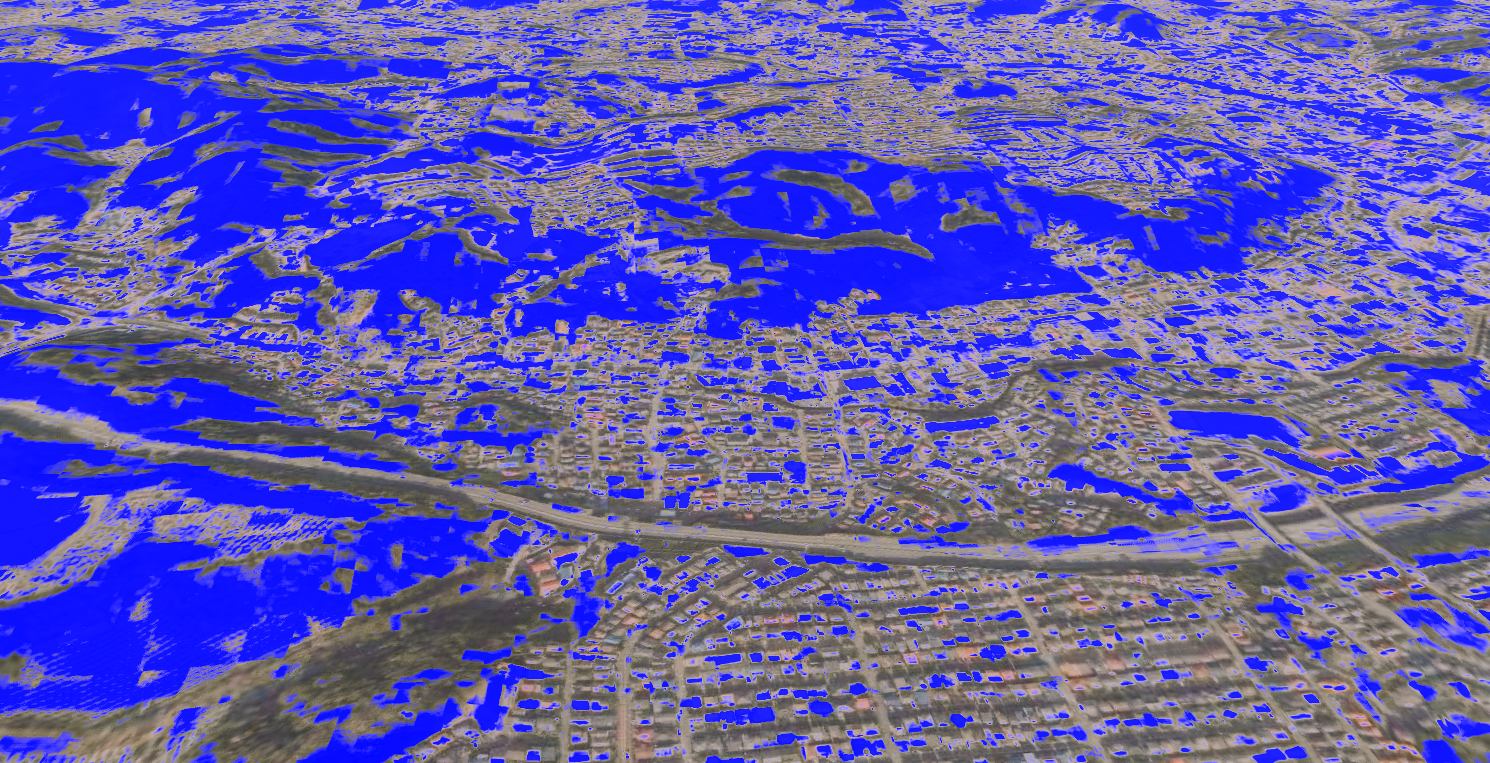
\includegraphics[height=4cm,width=5.5cm]{figures/snowArea2.PNG}}
    \subcaptionbox{}{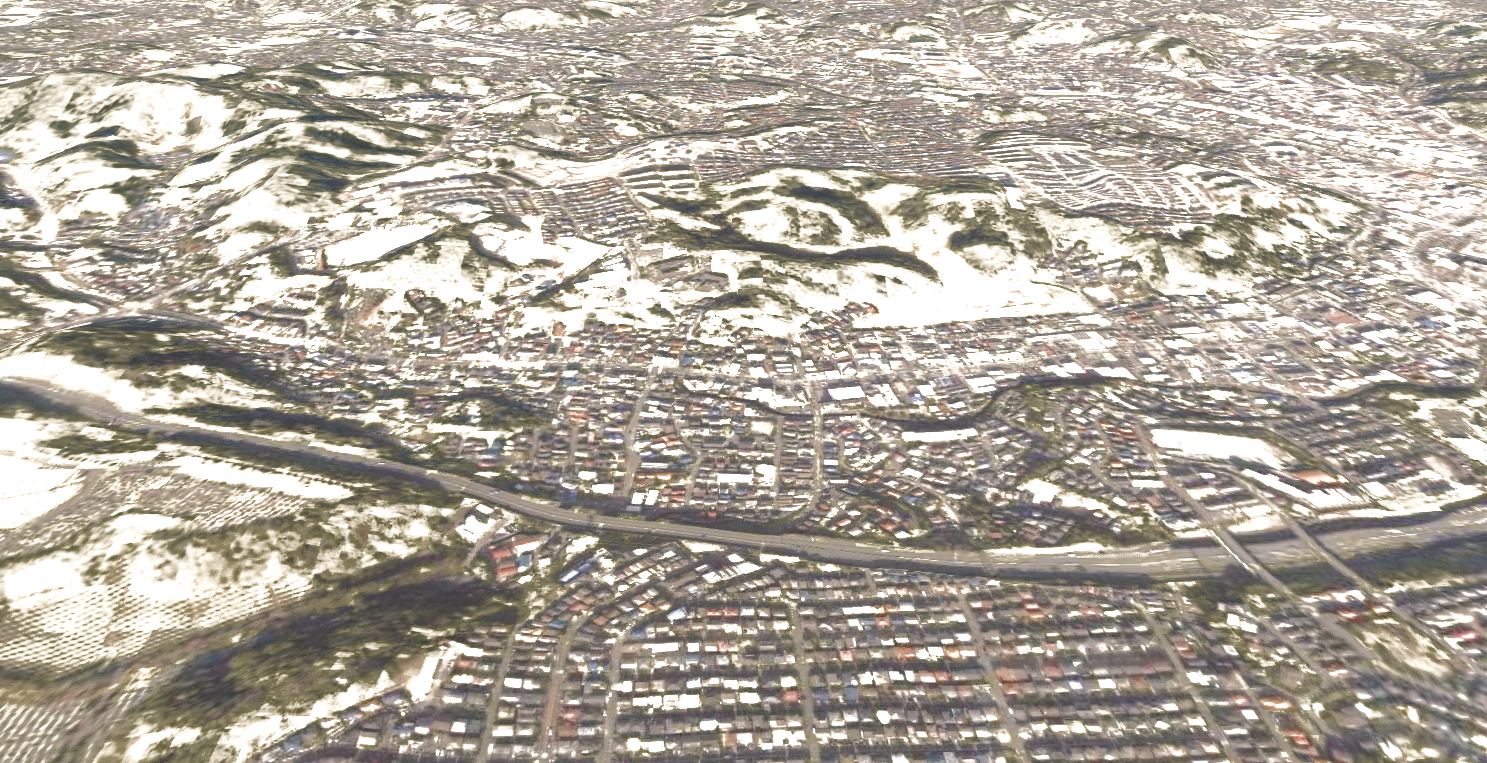
\includegraphics[height=4cm,width=5.5cm]{figures/snowy2.PNG}} \\
    \caption{冬季积雪效果:(a).覆雪区域(b).覆雪效果}
\end{figure}
本方法使用统一的输入色进行调色,可以在植被分布规律相同的局部取得较好的效果,但在植被分布规律不同的大规模地域上可能存在局限性。另外,此方法建立在对颜色信息的提取与分析上,由于卫星影像分辨率问题和阴影问题,在影像阴影的部分对语义的识别不够好,且随着地形块的层级切换,调色效果也会随着地形块所使用纹理数据而产生变化。\par
\section{渲染效率及效果优化}
\paragraph{三向贴图}
过程式建模常见的问题是难以为模型生成适当纹理展开的UV坐标,标准地形纹理映射方案在所有朝向的网格上固定沿着Y轴投影,用XZ坐标代替UV坐标进行纹理映射。这种方法在表面法线基本与投影轴平行的情况下可以有较好的表现,但表面法线与投影轴不对齐时,如地表纹理覆盖在坡度较陡的山地地形上时,经常形成拉伸和接缝的视觉效果。\par
三向贴图(Tri-planar mapping)是一种产生三维空间的平面上纹理坐标的纹理投影方法。沿着X、Y和Z轴用平面映射一个纹理三次,然后根据面片角度在这三个样本之间混合,可缓解地形陡坡上的拉伸效应,消除贴图对UV和切线方向的依赖。用面片法向量来计算三个投影的权值时需使用法向量的绝对值,因为一个曲面可以朝向负方向。为使权值的总和是1.0,最后通过除以各分量总和来进行标准化。本系统中使用三向贴图技术生成地表纹理UV的效果如图5.12所示:\par
\begin{figure}[H]
    \centering
    \subcaptionbox{}{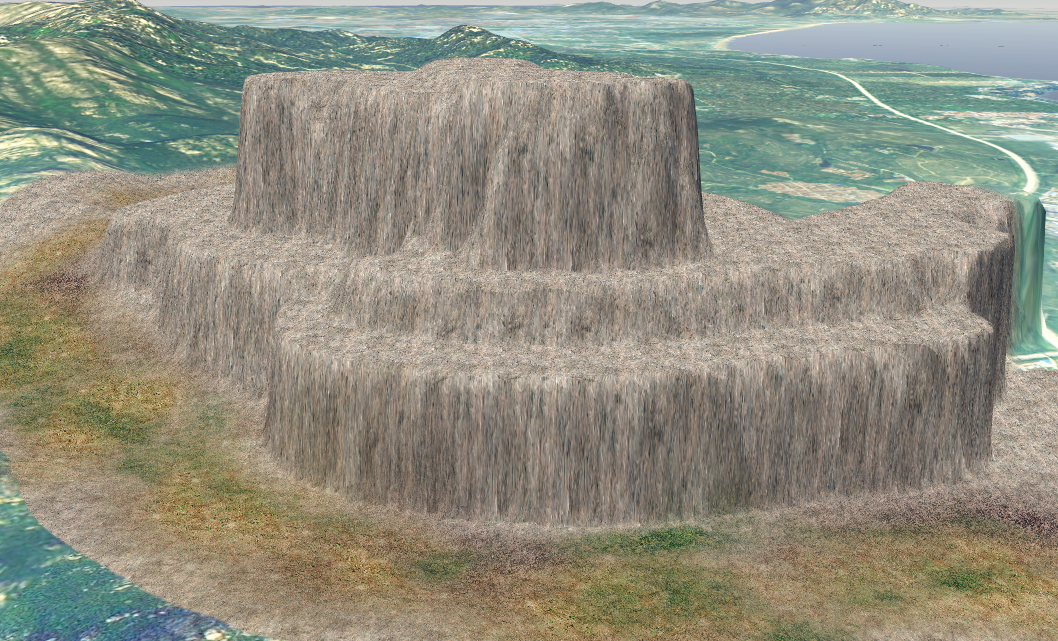
\includegraphics[height=4cm,width=6.5cm]{figures/tribefore.PNG}}
    \subcaptionbox{}{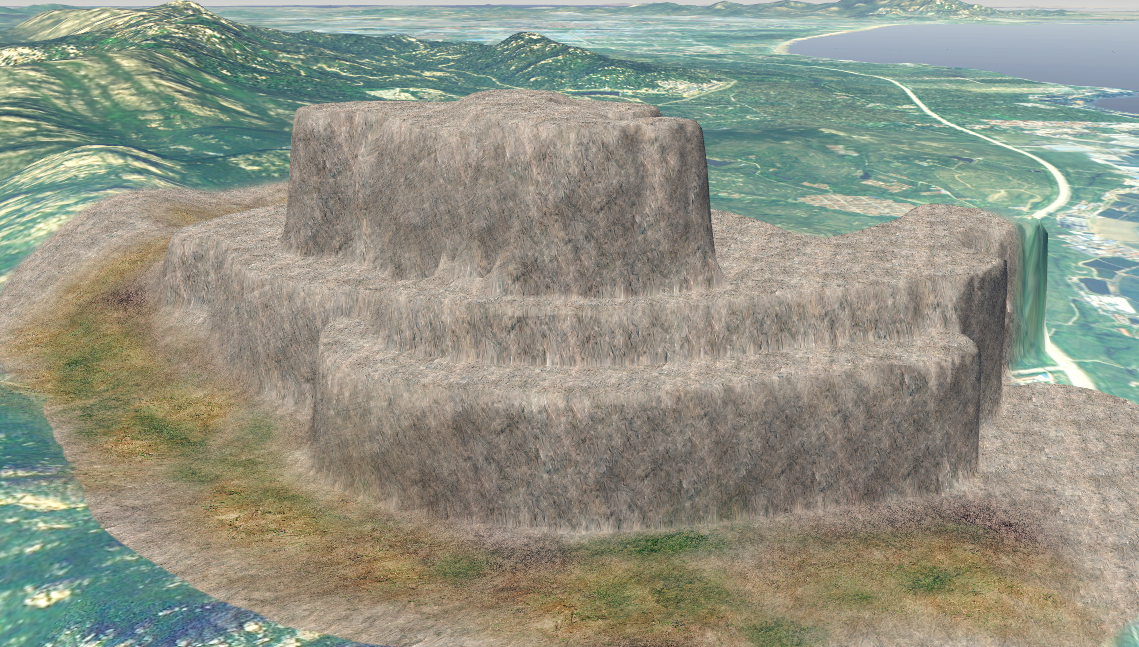
\includegraphics[height=4cm,width=6.5cm]{figures/triplanar.PNG}} \\
    \caption{三向贴图效果:(a).开启前垂直面拉伸现象严重(b).开启后垂直面贴图效果得到了优化}
\end{figure}
在多分辨率地形上的实现,需要额外根据当前层级的变化,对地形梯度的采样距离进行倍数修正,使不同层级的采样距离相等。
\paragraph{临时蒙版数据}
当异步对蒙版数据进行请求时,需要经过过滤器以应用所有编辑操作,当编辑操作较多,且涉及多个图层时,对于第一次请求到的块会产生很多分配数据、拷贝数据、过滤数据的时间开销,从而在视觉上产生较长时间的闪烁。对此,本文的改进之一是在数据未准备好时尝试构造临时蒙版数据,并增加了一个LRU队列用于保存临时构造产生的数据缓存。\par
根据子块与父块的索引可以推知子块在父块中的位置,因此可以将管理父块蒙版数据的智能指针赋给子块,并在着色器中根据子块在父块中的位置设置UV偏移量,从而在子块的位置用父块的数据正确的绘制。将使用了父块蒙版数据的缓存块称为临时块,当请求某地形块蒙版数据时,如没有确切的返回该块数据,则为该块构造一个临时数据用于绘制。由于直接使用了父块蒙版数据,构造临时数据的开销非常小,使请求蒙版数据块时卡顿闪烁的视觉效果得到了改善。

\section{结果分析}
本文设计的纹理编辑器界面如下图所示:\par
\begin{figure}[htb]
    \centering
    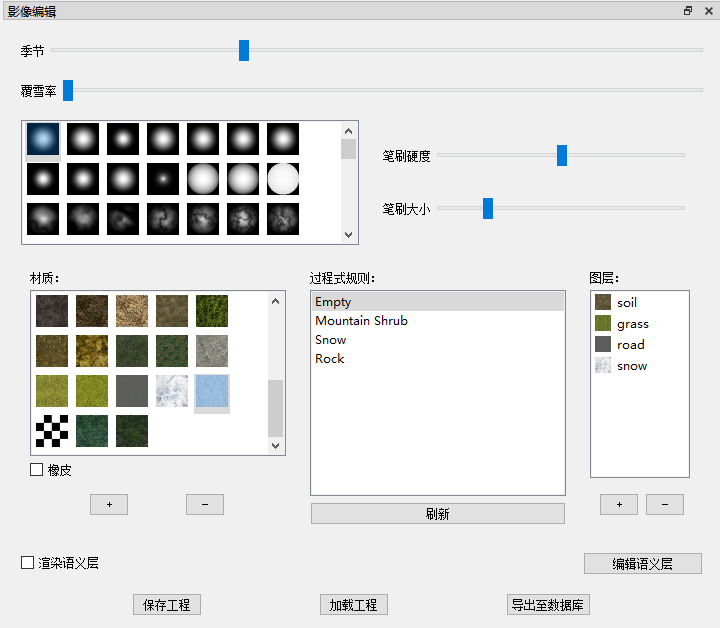
\includegraphics[height=9.8cm ,width=11.2cm]{figures/maskinterface.PNG}
  \caption{地表纹理编辑器界面}
  \end{figure}
编辑器预置了一套包含草地、泥土、沙地、荒地、雪地等材质的材质库(图5.13中间左侧材质栏),提供了若干种形状的笔刷(图5.13中间上方笔刷栏),预置笔刷编辑效果如图5.14所示。编辑地表纹理时,用户需要选中材质、笔刷和图层,每次编辑只应用在一个图层内。点击按钮创建新图层或删除图层,在图层列表项上双击可以改变创建时自动生成的图层名。选中图层后再点选材质可以对该图层所使用的材质进行更改,绘制时图层栏中的图层按创建顺序从下至上的叠加显示,按蒙版数据中保存的透明度对多种纹理材质进行混合。通过选中预置的规则(图5.13中间过程式规则一栏),用户可以简单的使某种纹理材质以符合其分布特征的方式绘制在地表上。\par
实现过程中,本文参考了ViWo中旧有的纹理编辑器,旧编辑器使用了与地形模块不同的地形数据结构,因此未能集成到系统中。本文的编辑器在笔刷模板、笔刷数据计算、用户界面等方面借鉴了旧编辑器,但实现方式上有很大的不同。旧编辑器为了简化编辑流程,设置了编辑状态与普通状态切换的步骤,切换入编辑状态后只显示以当前视点为中心的固定数量的地形块,相对来说操作不够简便,用户不能从不同的层级进行编辑和观察。本文实现的纹理编辑器与高程编辑器使用了相同的架构,架构上更加清晰,更易维护,并支持了在多层级地形块上的连续编辑。除此之外,加强了对图层的管理,提供了新建图层、图层命名、删除图层等操作;加强了材质的管理,可以使用复合材质,并动态的从本地磁盘中添加材质到编辑器;增加了使用高程规则的过程式编辑功能。完整的场景构建效果可参考附录中提供的三个地形场景。\par

\begin{figure}[H]
    \centering
    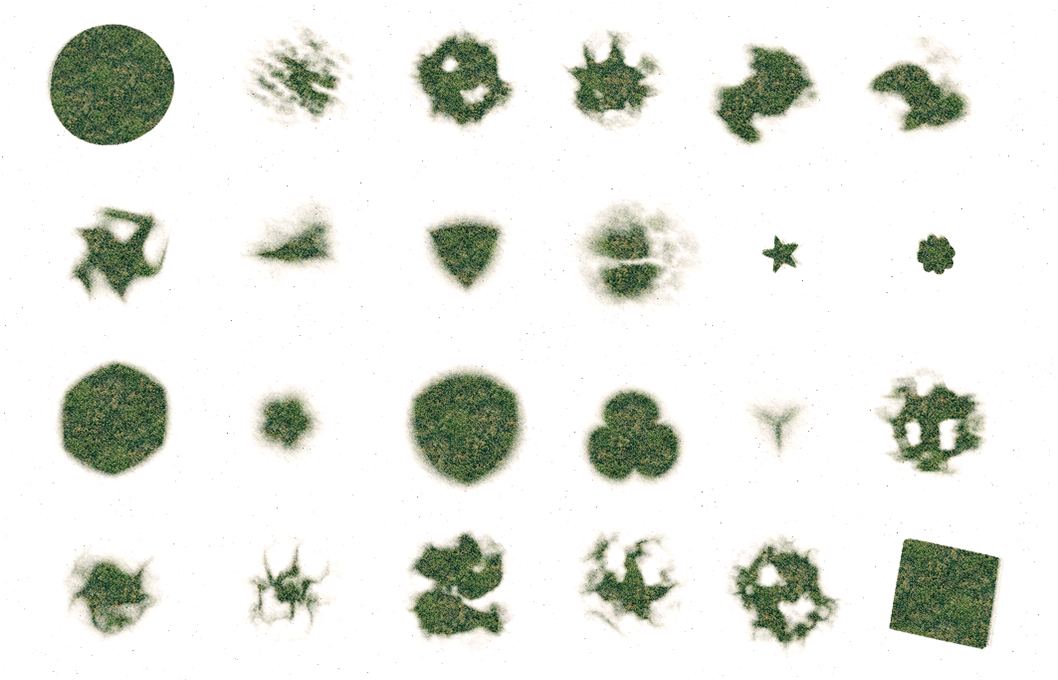
\includegraphics[height=4.2cm,width=6.2cm]{figures/brushEffect.jpg}
    \caption{预置的部分笔刷在系统中的编辑效果}
\end{figure}

对每帧产生固定时间开销的贴花效果和季节调整效果,本文进行了时间开销测试,测试方法是使用固定的摄像机漫游路线,记录开启和关闭效果后,绘制阶段CPU和GPU的时间开销,两次取平均。本文所使用的硬件信息详见附录,测试结果如表5.1所示,可以观察到开启贴花和季节调整对时间开销的影响非常小:
\begin{table}[h]
\caption{贴花和季节调整时间开销测试}  
\begin{tabularx}{15cm}{llll}  
\hline  
&关闭效果(ms)&开启贴花效果(ms)&开启季节调整效果(ms)\\
\hline
%S-GPU&0.058186&0.074827&0.06307\\
%\hline
GPU& 0.27425&0.354108&0.301634 \\
\hline
%S-CPU& 0.469164&0.525735&0.505344     \\
%\hline
CPU&0.605974&0.681484&0.672265    \\
\end{tabularx}  
\end{table}

\section{本章小结}
本章首先提出以笔刷为工具,以纹理Splatting技术进行纹理融合的纹理编辑方案,并说明了其优点。随后详细介绍了在大规模地形上实施多图层笔刷纹理编辑的方案。并针对内陆湖泊河流编辑效果不良的问题,提出了一种用复合纹理材质实现湖泊和河流效果的方法。为了提高编辑效率和真实感,提出了一种基于高程规则的纹理笔刷,可以通过简单的涂抹使编辑结果满足用户自定义的高程规则,创造复杂、具有真实感的效果。 \par
本章还提出了地表纹理使用的卫星影像数据分辨率低,携带信息量有限的问题,并针对该问题提出了基于颜色分析对低分辨率的卫星影像进行增强的方法。通过贴花技术为地表纹理添加细节,通过对卫星影像色调的改变丰富了卫星影像的内容,以较低的资源占用率,使粗糙卫星影像的在地形表面的贴图效果得到了提升。\par
最后,对地表纹理渲染中用到的效果和效率优化方法进行了说明。